% arara: clean: { files: [thesis.aux, thesis.bbl, thesis.blg, thesis.dvi, thesis.fdb_latexmk, thesis.fls, thesis.idx, thesis.ilg, thesis.ind, thesis.lof, thesis.log, thesis.lot, thesis.nlo, thesis.nls, thesis.out, thesis.pdf, thesis.ps, thesis.toc]}
% arara: latex:  { shell: yes }
% arara: bibtex
% arara: nomencl
% arara: latex
% arara: makeindex
% arara: latex:  { shell: yes }
% arara: dvips
% arara: ps2pdf

% ******************************* PhD Thesis Template **************************
% Please have a look at the README.md file for info on how to use the template

\documentclass[a4paper,12pt,times,numbered,print,index]{Classes/PhDThesisPSnPDF}

% ******************************************************************************
% ******************************* Class Options ********************************
% *********************** See README for more details **************************
% ******************************************************************************

% `a4paper'(The University of Cambridge PhD thesis guidelines recommends a page
% size a4 - default option) or `a5paper': A5 Paper size is also allowed as per
% the Cambridge University Engineering Deparment guidelines for PhD thesis
%
% `11pt' or `12pt'(default): Font Size 10pt is NOT recommended by the University
% guidelines
%
% `oneside' or `twoside'(default): Printing double side (twoside) or single
% side.
%
% `print': Use `print' for print version with appropriate margins and page
% layout. Leaving the options field blank will activate Online version.
%
% `index': For index at the end of the thesis
%
% `draft': For draft mode without loading any images (same as draft in book)
%
% `draftmode': Special draft mode with line numbers, images, and water mark with
% timestamp and custom text. Position of the text can also be modified.
%
% `abstract': To generate only the title page and abstract page with
% dissertation title and name, to submit to the Student Registry
%
% `chapter`: This option enables only the specified chapter and it's references
%  Useful for review and corrections.
%
% ************************* Custom Page Margins ********************************
%
% `custommargin`: Use `custommargin' in options to activate custom page margins,
% which can be defined in the preamble.tex. Custom margin will override
% print/online margin setup.
%
% *********************** Choosing the Fonts in Class Options ******************
%
% `times' : Times font with math support. (The Cambridge University guidelines
% recommend using times)
%
% `fourier': Utopia Font with Fourier Math font (Font has to be installed)
%            It's a free font.
%
% `customfont': Use `customfont' option in the document class and load the
% package in the preamble.tex
%
% default or leave empty: `Latin Modern' font will be loaded.
%
% ********************** Choosing the Bibliography style ***********************
%
% `authoryear': For author-year citation eg., Krishna (2013)
%
% `numbered': (Default Option) For numbered and sorted citation e.g., [1,5,2]
%
% `custombib': Define your own bibliography style in the `preamble.tex' file.
%              `\RequirePackage[square, sort, numbers, authoryear]{natbib}'.
%              This can be also used to load biblatex instead of natbib
%              (See Preamble)
%
% **************************** Choosing the Page Style *************************
%
% `default (leave empty)': For Page Numbers in Header (Left Even, Right Odd) and
% Chapter Name in Header (Right Even) and Section Name (Left Odd). Blank Footer.
%
% `PageStyleI': Chapter Name next & Page Number on Even Side (Left Even).
% Section Name & Page Number in Header on Odd Side (Right Odd). Footer is empty.
%
% `PageStyleII': Chapter Name on Even Side (Left Even) in Header. Section Number
% and Section Name in Header on Odd Side (Right Odd). Page numbering in footer


% ********************************** Preamble **********************************
% Preamble: Contains packages and user-defined commands and settings
% ******************************************************************************
% ****************************** Custom Margin *********************************

% Add `custommargin' in the document class options to use this section
% Set {innerside margin / outerside margin / topmargin / bottom margin}  and
% other page dimensions
\ifsetCustomMargin
  \RequirePackage[left=37mm,right=30mm,top=35mm,bottom=30mm]{geometry}
  \setFancyHdr % To apply fancy header after geometry package is loaded
\fi

% *****************************************************************************
% ******************* Fonts (like different typewriter fonts etc.)*************

% Add `customfont' in the document class option to use this section

\ifsetCustomFont
  % Set your custom font here and use `customfont' in options. Leave empty to
  % load computer modern font (default LaTeX font).
  \RequirePackage{helvet}
\fi

% *****************************************************************************
% **************************** Custom Packages ********************************

% ************************* Algorithms and Pseudocode **************************

%\usepackage{algpseudocode}
\usepackage{listings}

% ********************Captions and Hyperreferencing / URL **********************

% Captions: This makes captions of figures use a boldfaced small font.
%\RequirePackage[small,bf]{caption}

\RequirePackage[labelsep=space,tableposition=top]{caption}
\renewcommand{\figurename}{Fig.} %to support older versions of captions.sty


% *************************** Graphics and figures *****************************

%\usepackage{rotating}
\usepackage{wrapfig}

% Uncomment the following two lines to force Latex to place the figure.
% Use [H] when including graphics. Note 'H' instead of 'h'
%\usepackage{float}
%\restylefloat{figure}

% Subcaption package is also available in the sty folder you can use that by
% uncommenting the following line
% This is for people stuck with older versions of texlive
%\usepackage{sty/caption/subcaption}
\usepackage{subcaption}


% ********************************** Tables ************************************
\usepackage{booktabs} % For professional looking tables
\usepackage{multirow}

%\usepackage{multicol}
%\usepackage{longtable}
%\usepackage{tabularx}


% ***************************** Math and SI Units ******************************

\usepackage{amsfonts}
\usepackage{amsmath}
\usepackage{amssymb}
\usepackage{siunitx} % use this package module for SI units
\usepackage[euler]{textgreek}

% ******************************* Line Spacing *********************************

% Choose linespacing as appropriate. Default is one-half line spacing as per the
% University guidelines

%\doublespacing
%\onehalfspacing
\singlespacing


% ************************ Formatting / Footnote *******************************

% Don't break enumeration (etc.) across pages in an ugly manner (default 10000)
%\clubpenalty=500
%\widowpenalty=500

%\usepackage[perpage]{footmisc} %Range of footnote options


% *****************************************************************************
% *************************** Bibliography  and References ********************

%\usepackage{cleveref} %Referencing without need to explicitly state fig /table

% Add `custombib' in the document class option to use this section
\ifuseCustomBib
   \RequirePackage[square, sort, numbers, authoryear]{natbib} % CustomBib

% If you would like to use biblatex for your reference management, as opposed to the default `natbibpackage` pass the option `custombib` in the document class. Comment out the previous line to make sure you don't load the natbib package. Uncomment the following lines and specify the location of references.bib file

%\RequirePackage[backend=biber, style=numeric-comp, citestyle=numeric, sorting=nty, natbib=true]{biblatex}
%\bibliography{References/references} %Location of references.bib only for biblatex

\fi

% changes the default name `Bibliography` -> `References'
\renewcommand{\bibname}{References}


% *****************************************************************************
% *************** Changing the Visual Style of Chapter Headings ***************
% This section on visual style is from https://github.com/cambridge/thesis

% Uncomment the section below. Requires titlesec package.

%\RequirePackage{titlesec}
%\newcommand{\PreContentTitleFormat}{\titleformat{\chapter}[display]{\scshape\Large}
%{\Large\filleft{\chaptertitlename} \Huge\thechapter}
%{1ex}{}
%[\vspace{1ex}\titlerule]}
%\newcommand{\ContentTitleFormat}{\titleformat{\chapter}[display]{\scshape\huge}
%{\Large\filleft{\chaptertitlename} \Huge\thechapter}{1ex}
%{\titlerule\vspace{1ex}\filright}
%[\vspace{1ex}\titlerule]}
%\newcommand{\PostContentTitleFormat}{\PreContentTitleFormat}
%\PreContentTitleFormat


% ******************************************************************************
% ************************* User Defined Commands ******************************
% ******************************************************************************

% *********** To change the name of Table of Contents / LOF and LOT ************

%\renewcommand{\contentsname}{My Table of Contents}
%\renewcommand{\listfigurename}{My List of Figures}
%\renewcommand{\listtablename}{My List of Tables}

\lstdefinestyle{haskellStyle}{
	language=Haskell,
	numbers=left,
	stepnumber=1,
	numbersep=10pt,
	tabsize=4,
	showspaces=false,
	showstringspaces=false,
	basicstyle=\footnotesize,
	columns=flexible
}
\newcommand{\vecb}[1]{\vec{\mathbf{#1}}}
\newcommand{\matr}[1]{\mathbf{#1}}
\newcommand{\code}[1]{\lstinline{#1}}
\newcommand{\sep}{\hspace{50pt}}
\newcommand{\clash}{C$\lambda$aSH}
\newcommand{\matlab}{MATLAB} %\textsuperscript{\textregistered}
\providecommand{\e}[1]{\ensuremath{\times 10^{#1}}}

\newenvironment{itemizens}
{ 
	\vspace{-\topsep}
	\begin{itemize}
	\setlength{\itemsep}{0pt}
	\setlength{\parskip}{0pt}
	\setlength{\parsep}{0pt}     
}
{ 
	\end{itemize}
} 

\newenvironment{enumeratens}
{
	\vspace{-\topsep}
	\begin{enumerate}
	\setlength{\itemsep}{0pt}
	\setlength{\parskip}{0pt}
	\setlength{\parsep}{0pt}     
}
{ 
	\end{enumerate}                  
} 


% ********************** TOC depth and numbering depth *************************

\setcounter{secnumdepth}{2}
\setcounter{tocdepth}{2}


% ******************************* Nomenclature *********************************

% To change the name of the Nomenclature section, uncomment the following line

%\renewcommand{\nomname}{Symbols}


% ********************************* Appendix ***********************************

% The default value of both \appendixtocname and \appendixpagename is `Appendices'. These names can all be changed via:

%\renewcommand{\appendixtocname}{List of appendices}
%\renewcommand{\appendixname}{Appndx}

% ******************************** Draft Mode **********************************

% Uncomment to disable figures in `draftmode'
%\setkeys{Gin}{draft=true}  % set draft to false to enable figures in `draft'

% These options are active only during the draft mode
% Default text is "Draft"
%\SetDraftText{DRAFT}

% Default Watermark location is top. Location (top/bottom)
%\SetDraftWMPosition{bottom}

% Draft Version - default is v1.0
%\SetDraftVersion{v1.1}

% Draft Text grayscale value (should be between 0-black and 1-white)
% Default value is 0.75
%\SetDraftGrayScale{0.8}


%% Todo notes functionality
%% Uncomment the following lines to have todonotes.

%\ifsetDraft
%	\usepackage[colorinlistoftodos]{todonotes}
%	\newcommand{\mynote}[1]{\todo[author=kks32,size=\small,inline,color=green!40]{#1}}
%\else
%	\newcommand{\mynote}[1]{}
%	\newcommand{\listoftodos}{}
%\fi

% Example todo: \mynote{Hey! I have a note}


% ************************ Thesis Information & Meta-data **********************
% Thesis title and author information, refernce file for biblatex
% ************************ Thesis Information & Meta-data **********************
%% The title of the thesis
\title{Numerical mathematics on FPGAs using C\textlambda aSH}
%\texorpdfstring is used for PDF metadata. Usage:
%\texorpdfstring{LaTeX_Version}{PDF Version (non-latex)} eg.,
%\texorpdfstring{$sigma$}{sigma}

%% Subtitle (Optional)
\subtitle{Comparison to conventional solution methods}

%% The full name of the author
\author{Martijn Bakker}

%% Department (eg. Department of Engineering, Maths, Physics)
\dept{Committee: \\ 
	Dr.ir. J. Kuper \\ 
	Dr. R.M.J. van Damme \\ 
	Dr.ir. J. Broenink \\ 
	\vspace{150pt}	
	Computer Architecture for Embedded Systems
	Electrical Engineering, Mathematics and Computer Science (EEMCS)
}

%% University and Crest
\university{University of Twente}
%\crest{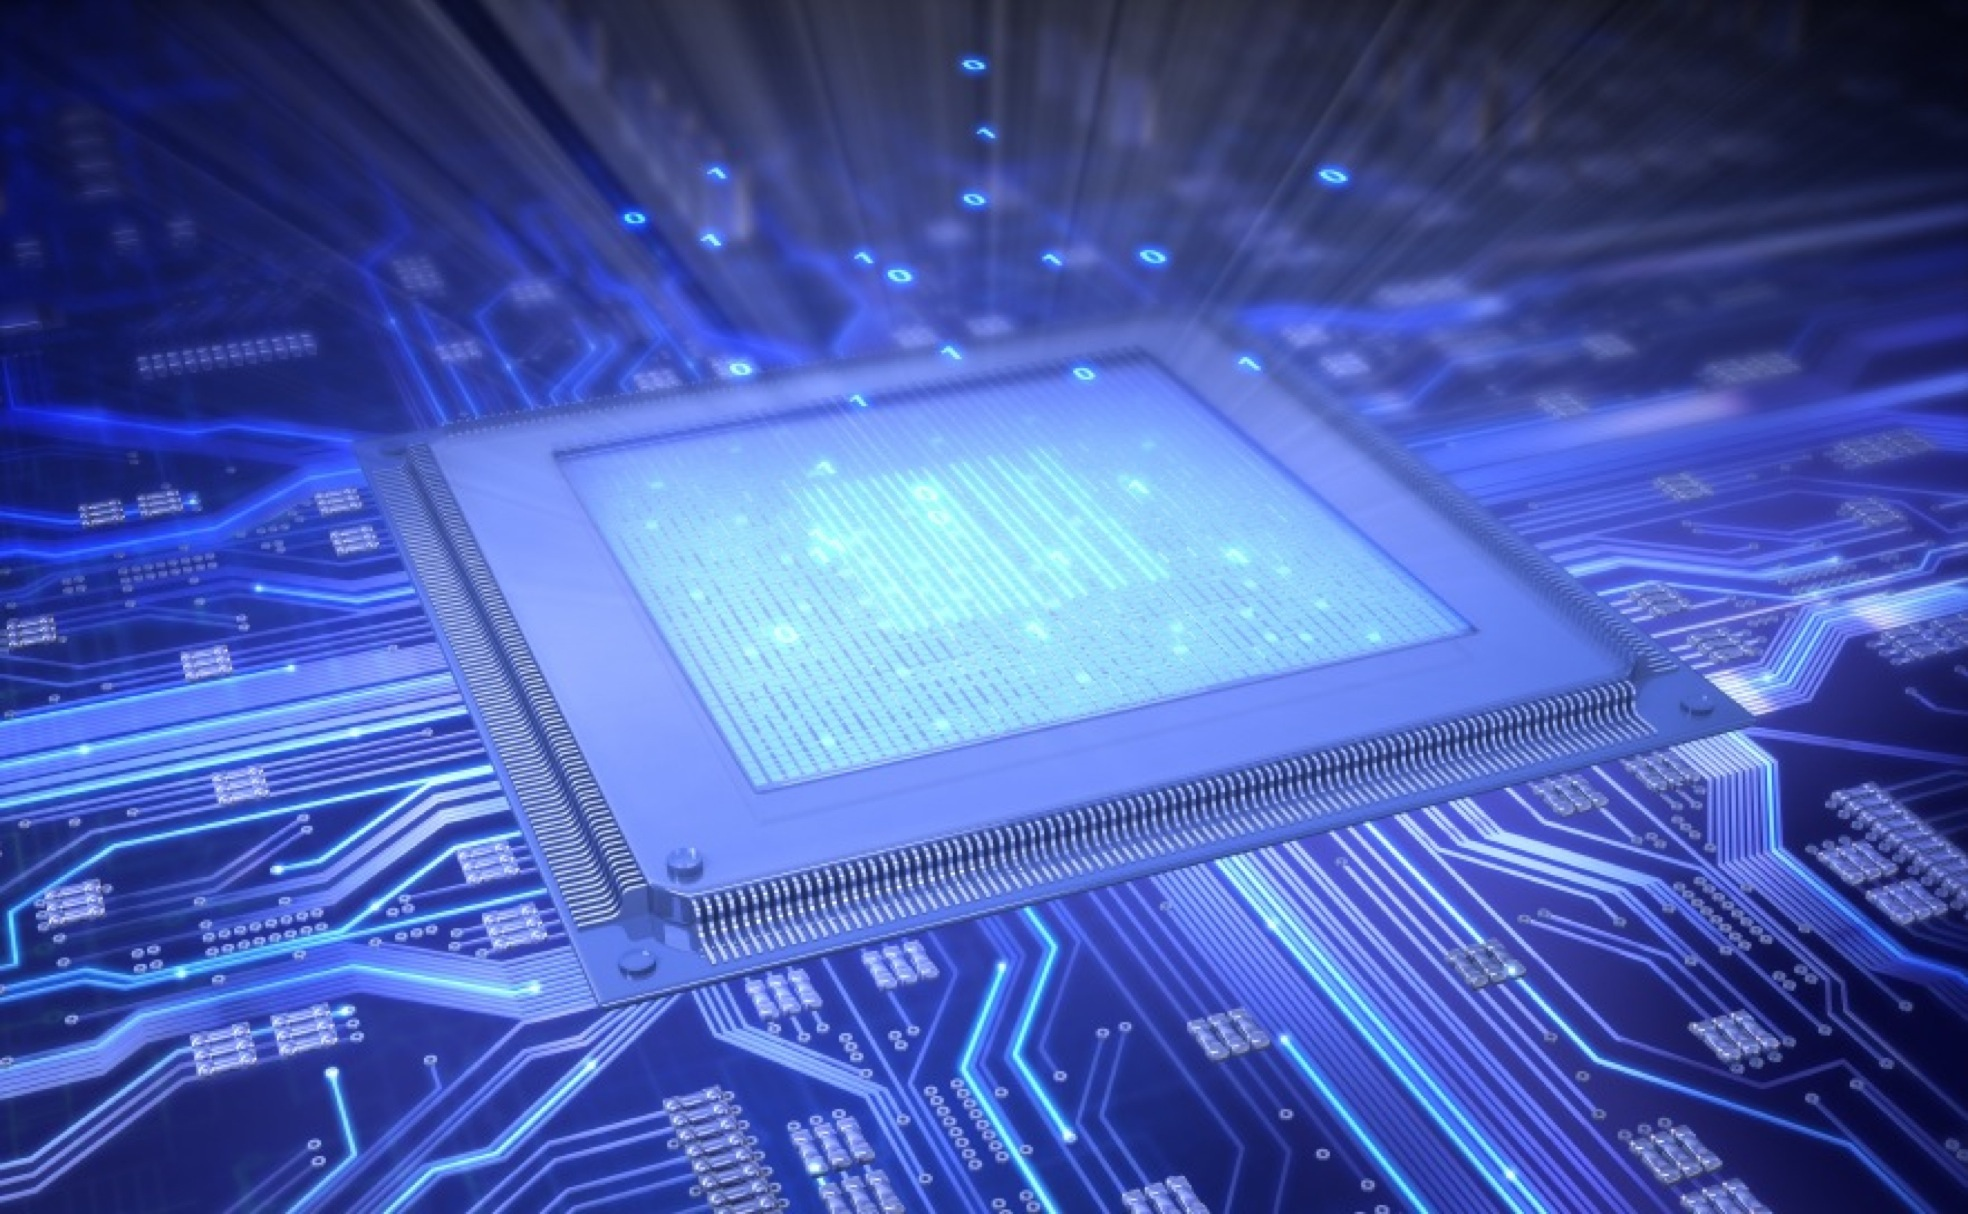
\includegraphics[width=\textwidth]{fpga_wallpaper}}

%% You can redefine the submission text:
% Default as per the University guidelines:
% ``This dissertation is submitted for the degree of''
\renewcommand{\submissiontext}{This thesis is submitted for the degree of}

%% Full title of the Degree
\degreetitle{Bachelor of Science}

%% College affiliation (optional)
\college{Advanced Technology}

%% Submission date
% Default is set as {\monthname[\the\month]\space\the\year}
\degreedate{July 2015} 

%% Meta information
\subject{LaTeX} \keywords{{LaTeX} {PhD Thesis} {Engineering} {University of Cambridge}}


% ***************************** Abstract Separate ******************************
% To printout only the titlepage and the abstract with the PhD title and the
% author name for submission to the Student Registry, use the `abstract' option in
% the document class.
\ifdefineAbstract
 \pagestyle{empty}
 \includeonly{Intro/abstract}
\fi

% ***************************** Chapter Mode ***********************************
% The chapter mode allows user to only print particular chapters with references
% Title, Contents, Frontmatter are disabled by default
% Useful option to review a particular chapter or to send it to supervisior.
% To use choose `chapter' option in the document class
\ifdefineChapter
	\includeonly{P1-Introduction/introduction,P2-Main/methods,P2-Main/results}
\fi

% ******************************** Front Matter ********************************


\begin{document}

\frontmatter

\begin{titlepage}
  \maketitle
\end{titlepage}





% *********************** Adding TOC and List of Figures ***********************

\begin{abstract}
Performing computations directly in hardware can be a very challenging task for a scientist or engineer only familiar with software, but there is much that can be gained in terms of power reduction and performance improvements using FPGAs. This thesis describes the process of implementing an accelerator in which the computational part is specified using the functional hardware description language \clash{} and discusses the feasibility of performing numerical mathematics on this accelerator by computing approximations to ordinary differential equations. The accelerator is capable of using the methods of Euler and Runge-Kutta (second order) to perform the approximations, but due to the use of a fixed-point number representation the accuracy suffers. The performance of the accelerator, implemented on a low-power, low-cost development FPGA: the Altera Cyclone V is 40\% worse than an i7-950, but the power usage of the accelerator is 2 orders of magnitude lower. 
\end{abstract}

% ************************** Thesis Acknowledgements **************************

\begin{acknowledgements}      
\begin{itemizens}
	\item Jan Kuper	- Introducing me to functional programming, \clash{} and giving feedback
	\item Christiaan Baaij - Creating \clash{} and answering related questions
	\item Ruud van Damme \& Jan Broenink - Feedback
	\item Rinse Wester - Input on configuring and using the Avalon bridges
\end{itemizens}

\end{acknowledgements}


\vfill

\begin{acronyms}
\begin{tabular}{>{\bfseries}l l}
	ASIC & Application-specific integrated circuit \\
	FPGA & Field-Programmable Gate Array \\
	CPU & Central Processing Unit \\
	%GPU & Graphics Processing Unit \\
	%GPGPU & General Purpose GPU \\
	DSP & Digital Signal Processing \\
	LED & Light Emitting Diode \\
	VHDL & VHSIC HDL \\
	VHSIC & Very High Speed Integrated Circuit \\
	HDL & Hardware Description Language \\
	SoC & System-on-Chip \\ 
	ODE & Ordinary Differential Equation \\
	HPS & Hard Processor System \\
	ARM & Advanced RISC Machine (CPU development company) \\
	RISC & Reduced Instruction Set Computer \\
	IP & Intellectual Property \\
	GUI & Graphical User Interface \\
\end{tabular}		
\end{acronyms}    

  

\tableofcontents

%\listoffigures
%\listoftables

\printnomencl

% ******************************** Main Matter *********************************
\mainmatter

\chapter{Introduction} 

\section{Solver theory -- TODO}

\subsubsection{Euler}
Take derivative, multiply with timestep, add to initial value, repeat until end.

\subsubsection{Runge-Kutta methods}
Take derivatives at some time points, multiply with proper coefficients, add all to intial value, repeat until end.

\subsubsection{Stability}

\section{What is FP -- TODO}
Should I add a section on this to make everything understandable to all readers?


\section{Using Haskell for numerical mathematics}
Functional languages have several properties which make them suitable for the purpose of solving problems in numerical mathematics. First and foremost, Haskell, being based on $\lambda$-calculus is very close to mathematics. The useful mathematical properties here are \textit{referential transparency}, easy \textit{partial function application} and being a \textit{declarative language}. 
Referential transparency implies that a variable only has a constant value which is the same everywhere in the program. This prevents that changing a variable might have influence on another computation as a side effect and it corresponds to mathematical notation. For instance, in an imperative programming like C you could write \code{i = i + 1}, which is a mathematical impossibility and therefore not allowed in Haskell. 
Partial function application is another very useful concept. Often in numerical mathematics, you want to create or process a function. You need a function that has another function as return value. For instance, take a function which requires two arguments. After only applying a single argument, the object returned still needs the second argument in order to compute the final value. This is exactly according to the definition of a function: An object that still needs arguments before being able to return its final value.
Being a \textit{declarative language} means that you write code that specifies what you want to accomplish, not how to get there. This concept is again borrowed from mathematics. You put in a set of function definitions and Haskell will figure out how to actually compute the value you request according to those definitions. This property of declarativity also has the result that Haskell is a very terse language whilst remaining easy to understand.
Secondly, Haskell has a very strong type system. The type system has three main advantages. It becomes very easy to swap out and replace functions as long as you make sure that the types are the same. The Haskell compiler will start to assert errors immediately whenever you feed it something which does not make sense or could be ambiguous which is very useful when writing programs. By having a look at the types of a Haskell program it becomes very straightforward to see what the program does and how it works, which is very useful when attempting to understand your own or someone else's code.
Lastly, a property which is often very important for numerical mathematics: Haskell is fast. According to the \textit{Computer Language Benchmarks Game} \cite{Bench}, Haskell is almost on par with Java and Fortran but significantly faster than Python and Matlab (not shown), two languages which are often used for numerical mathematics nowadays. There is still a performance gap of around a factor 3 between Haskell and C (the reference), hence if speed is of the absolute highest concern C is still a valid option.

\section{Numerical solutions of ODEs in Haskell}
\lstset{style=haskellStyle}

As mentioned before, the types in Haskell reveal lots of information about the structure and functionality of the program. The three main types constituting the numerical solver for ordinary differential equations are listed above.

\lstinputlisting[caption=Main types for the ODE solver, label=solvertypes, firstline=18]{../haskell/SolverTypes.hs}

\subsubsection{Equation}
In essence, a differential equation is a mapping (function) from a certain state of the system to the change of this system. This is also what the type signature of \code{Equation} signifies, a mapping from an \code{ODEState} to a \code{D_ODEState}. This generic set up allows the specification of any ODE for solving. The implementation in pure Haskell of a simple ODE is given in listing \ref{lst:eq_exponential}, which corresponds to the equation $x' = -x$. However, this representation is not very elegant and a lot of the code is performing unboxing of the types. Using property that this equation is linear, it is possible to use an utility method which takes as input a matrix and returns the Haskell differential equation function belonging to that matrix. The same can be done for heterogeneous linear systems using a different utility function, which does not only takes a matrix as input but also a list of functions representing the heterogeneous part of the equation. The example code for this can be seen in appendix \ref{app:haskellsolver}.

\lstinputlisting[caption=Example equation for exponential decay, label=lst:eq_exponential, firstline=11,lastline=14]{../haskell/SolverEquations.hs}

\subsubsection{SolveMethod}
The \code{SolveMethod} performs the actual computations on what the next value of the solution should be: the integration scheme. In order to obtain this next state, the scheme needs three input values: It needs information on the timing constraints of the solution, in this case it needs the time step. Furthermore, it needs the equation itself and it requires the state of the system at $t_{n}$ in order to be able to determine the state of the system at $t_{n+1} = t_{n} + \Delta t$.

The most straightforward integration scheme is called forward Euler, given in equation \ref{eq:forward_euler}. Listing \ref{lst:forward_euler} depicts the translation of the mathematical expression \ref{eq:forward_euler} to Haskell. Even though some list operations have been inserted (\code{zipWith} and \code{map}), the structure is still recognizable. It computes the change in state, multiplies this with the time step obtained in line 6 and adds the initial state in line 4. Lastly, the integration scheme returns the new state of the equation, consisting of a list of x-values and a corresponding time value. Implementations of different solvers (eg. 4th order Runge-Kutta) can be found in appendix \ref{app:haskellsolver}.

\lstinputlisting[caption=Example code for the forward Euler integration scheme, label=lst:forward_euler, firstline=9,lastline=15]{../haskell/SolverSolvers.hs}

\begin{equation}
\label{eq:forward_euler}
\vecb{x}(t + \Delta t) \approx \vecb{x}(t) + \frac{\mathrm d \vecb{x}(t)}{\mathrm d t}\Delta t
\end{equation}

\subsubsection{Solver}
The \code{Solver} function in listing \ref{lst:solver_frame} acts as the main interface to the program. You specify a \code{SolveMethod}, the \code{TimeSettings} (containing the time step and the time at which to stop solving), the equation itself and an initial condition. The \code{Solver} will then return a list of states of the system. As is very common in functional programming, the \code{Solver} has been defined recursively. Line 4 is where the magic happens: the solution list is defined to be the initial condition, followed by the solution list with the new state (computed by the integration scheme on line 6) as initial condition. Additionally, there is a comparison in line 7 which ends the recursion whenever the time of the solution exceeds the maximum time value, set in the \code{TimeSettings}.

The solutions of a wide range of equations, both linear and non-linear, both homogeneous and heterogeneous and using the input matrix utility functions have been plot with suitable initial conditions to show their behavior in figure \ref{fig:solver_example}.

\lstinputlisting[caption=The main controlling function, label=lst:solver_frame, firstline=14,lastline=20]{../haskell/Solver.hs}

\begin{figure}[h!]
	\centering
	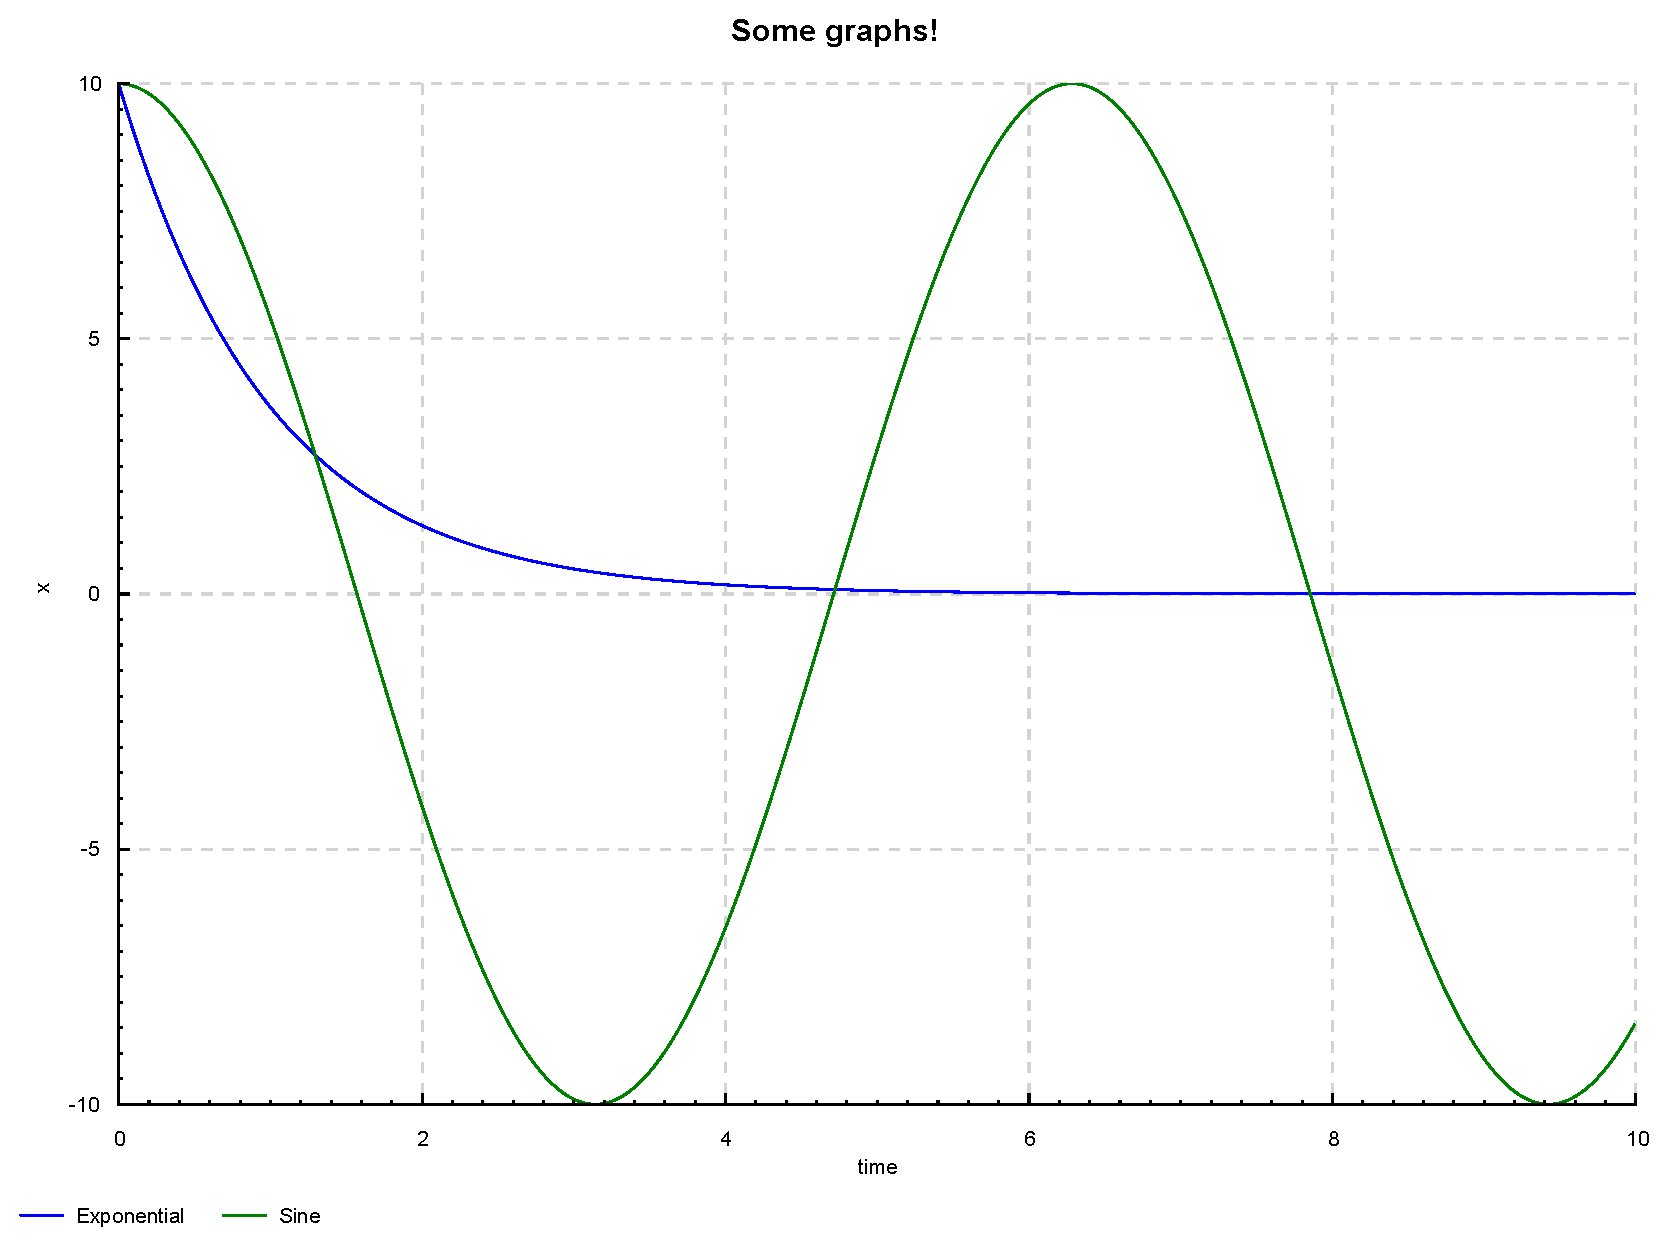
\includegraphics[width=\textwidth]{../haskell/output.pdf}
	\caption{Graphs}
	\label{fig:solver_example}
\end{figure}

\begin{align}
\text{Exponential}\sep{}			x(t)' &= -x(t)  \\
\text{Simple harmonic}\sep{}		x(t)'' &= -x(t) \\
\text{Cosine hyperbolic}\sep{}		x(t)' &= \frac{\sqrt{x(t)^{2} - a^{2}}}{a} \\
\text{Simple harmonic}\sep{}		\vecb{x}(t)' &= \begin{bmatrix} 0 & 1 \\ -1 & 0 \\ \end{bmatrix}\vecb{x}(t) \\
\text{Simple forced harmonic}\sep{}	\vecb{x}(t)' &= \begin{bmatrix} 0 & 1 \\ -1 & 0 \\ \end{bmatrix}\vecb{x}(t) + \begin{bmatrix} \sin{(t)} \\ e^{-t} \\ \end{bmatrix}
\end{align}




\section{Conversion to Mealy Machines / C$\lambda$aSH -- TODO}

Changes to:
\begin{itemize}
	\item Equation : numerical types (fixed point) - what operations would be supported in VHDL (hard to do nonlinear operators, sqrt(), sin(), cos(), tan()) - 
	\item SolutionMethod - becomes transition function of the mealy machine
	\item Solver - keeping track of the state of the solution - responsible for loading the data from the AXI-bridge to the HPS - responsible for outputting the data to the HPS for storage/processing/streaming
\end{itemize}

\iffalse
\begin{equation}
\frac{\mathrm d \vecb{x}(t)}{\mathrm d t} = f(\vecb{x}) + g(t)
\end{equation}

\begin{equation}
\frac{\mathrm d \vecb{x}(t)}{\mathrm d t} = \matr{A} \vec{x} + g(t)
\end{equation}
\fi

\section{FPGAs -- TODO}
\begin{itemize}
	\item What are FPGAs used for?
	\item Why should I care about FPGAs
	\item What is the current workflow for programming FPGAs
\end{itemize}


\section{Data transfer -- TODO}
\chapter{Methods}
This chapter contains a description of the methods used in describing the hardware on the FPGA side using \clash{} and VHDL. The description of the host-side (HPS) programming is included in appendix \ref{app:data_io}, as even though this part of the project is crucial for obtaining results, it is merely tangential to the project goals. The methods are ordered chronologically in order to properly describe the process that lead to the FPGA side programming used in chapter \ref{s:results}. This approach has as side effect that the explanation of the source code is evaluated lazily: only whenever necessary. Therefore the IO system is only covered after testing and synthesis, as it is not yet needed before.

\section{Overall structure}
In any reasonably complex project it pays off to keep a clear structure: it improves understandability and allows for easier debugging. For simple projects in \clash{}, the structure would be uniquely determined by the HDL generated by \clash{}, but this project also relies on other sources of HDL. Most noteworthy, the interface between the HPS and the FPGA; these signals are very specific to the type of the FPGA and the interconnects it has to the HPS. Luckily, the vendor (Altera) provides a way to generate HDL (the QSys system) in order to create a bridge from the host code running on the HPS to the programmable hardware, the FPGA. This process is described in appendix \ref{app:data_io_setup}. After configuring the bridge, VHDL can be generated and we are left with an instantiable VHDL component. However, even though \clash{} is capable of instantializing external IP components written in VHDL \cite{CLaSHBlogTut}, the most sensible way of implementing such a structure (due to the easy extensibility) is by writing a specific connecting component in VHDL, which can instantiate the \clash{}-generated VHDL. The only responsibility of the connecting component is to distribute and forward signals: it should not perform any computation. It would be a straightforward process of generating such a connecting component based on the signal names in the top-level entities of the components it instantiates, however, due to the fact that it does not change for different designs and it is not very large, the connecting component has been written by hand in VHDL. Figure \ref{f:large_structure} depicts an overview schematic of the complete system, including both the FPGA and HPS side.

\begin{figure}[h]
	\centering
	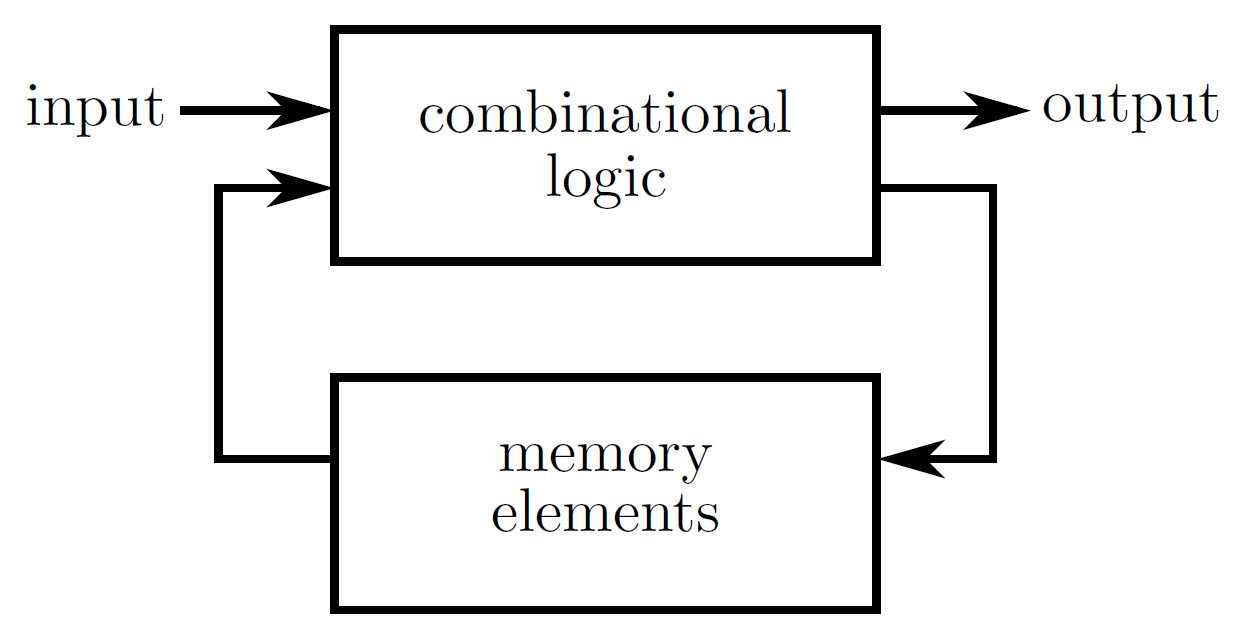
\includegraphics[width=\textwidth]{mealy_machine}
	\caption{TODO FIX ENTER GRAPHIC OF STRUCTURE WITH ILLUSTRATOR}
	\label{f:large_structure}
\end{figure}

\section{External types}
Usually, one of the first things to do when setting up a Haskell project is defining types, and using \clash{} forms no difference. It is especially useful to start by defining an input and an output signal. In a project with simple IO requirements the input and output signals would map straight to switches, keys and LEDs for testing purposes, but as the goal is to write data from the host system into the FPGA registers, the input and output signals will be a lot more complicated. The input and output signals from the \clash{}-generated VHDL top entity are shown in listing \ref{lst:clash_io_types}. The input consists of three separate channels: a bidirectional control channel, the actual input channel and some input needed for the output channel. It might appear strange that the output channel requires input, but this is necessary as the communications adhere to a strict master-slave pattern, in which the HPS is the master and the FPGA the slave. The HPS has to indicate whenever it wants to receive the FPGA output (by specifying an address (\code{out_address}) and setting the \code{out_read}-bit). As a consequence of the strict master-slave protocol, there are a lot less output signals than input signals: only the control and output channel can output data. Lastly, there are the keys, switches and LEDs as additional input and output signals. This concludes the type signatures of the input and output signals in \clash{}-Haskell. However, as the goal is to generate actual VHDL, \clash{} requires some additional information for the naming of the ports of the topEntity of the VHDL module. This is specified using the \code{topEntity}-annotation. In this case this annotation is not very interesting and it's merely a restatement of the input and output signal names, but when the \clash{}-generated VHDL should instantiate other VHDL-modules or use multiple clocks, the annotation can become more complex. It is shown in listing \ref{lst:clash_topentity}. 

\lstinputlisting[caption=Input and output signals for CλaSH, label=lst:clash_io_types, firstline=5,lastline=21]{../clash/SolverTypes.hs}
\lstinputlisting[caption=Signal names\, used in the CλaSH-generated topEntity VHDL module, label=lst:clash_topentity, firstline=8,lastline=29]{../clash/Solver.hs}

\section{Internal types}
So far the external types of the \clash{}-code have been covered, but the real work is done by the internal types: the types that keep track of the state of the system and allow it to do useful work. In order to allow for easy modifications to the types upon which the FPGA operates, they have been defined once and have been referenced everywhere else. This in combination with the property of the higher-order functions in \clash{} that they can operate on all vectors, regardless of length ensures that changing some internal types will not break the program.

\subsection{Internal number representation}
The solvers main data type is \code{type Data = SFixed 8 24}. The constructor \code{SFixed 8 24} stands for a signed fixed-point number, with 8 integer bits and 24 fractional bits. It uses the 2's complement signed number representation, meaning that an 8-bit integer part is capable of representing the integers in the range $[-128..127]$. The 24 fractional bits give this number representation a smallest representable unit of $2^{-24}$. This results in accuracy up to the 7th decimal place, which is similar to the IEEE 754 single precision floating point standard. The main reason for the use of fixed point integers is that \clash{} does not support floating point numbers yet, but additionally, fixed point representations are less demanding on FPGA area and result in a shorter critical path. Furthermore, the reason for choosing the total width of the number representation to be 32-bits is purely convenience: the input and output bridges are also 32 bits wide which allows you to send a single number per write or read. Lastly, the \code{UInt} type acts as number representation in cases where only positive integer values are required, for instance in counters.

\subsection{SystemConstants and SystemState}
The \code{SystemConstants} keep track of the variables that do not change during the process of solving the ODE. It consists of a variety of constants that need values for the integration scheme (\code{maxtime}, \code{timestep} and \code{maxstep}). Furthermore, it may contain custom constants, which are passed to the equation to be approximated. This setup allows for (limited) changes to the equation by changing the constants at run-time without the time-consuming requirement of recompiling the entire FPGA side of the project.

Moving on to the data type which responsible for keeping track of the state of the system: the \code{SystemState}. This type has two fields: the \code{ODEState}, which is has the exact same function as the similarly named type in section \ref{s:numsolHaskell}: it keeps track of the values and the time in the numerical solver. It does this using a \code{valueVector} (of type \code{Vec 4 Data}) and a \code{time} variable (of type \code{Data}). The main difference between the type of the \code{ValueVector} in this implementation of \code{ODEState} and the one in section \ref{s:numsolHaskell} is that this one uses a vector instead of a list. In Haskell, lists can have any length (including infinite) whereas the \clash{}-vectors have a fixed length. This property is very important when generating VHDL, as all vector lengths have to be immutable and known at compile-time in order to compile the higher-order Haskell functions (eg. map) to VHDL and afterwards to hardware. 

The second field of the \code{SystemState} is a counter called \code{step}. Together with the \code{maxstep} field in \code{SystemConstants}, these govern the amount of output generated from the FPGA. A more elaborate explanation of the generation of output can be found in section \ref{s:compute}.

\lstinputlisting[caption=Internal state variables for CλaSH, label=lst:clash_internal_types, firstline=23,lastline=45]{../clash/SolverTypes.hs}

\section{Implementation of equations and integration schemes}
The \clash{}-implementations of the equations and integration schemes can be very similar to the implementations in plain Haskell, from section \ref{s:numsolHaskell}. However, \clash{} does not support any special operations yet (exponentiation, trigonometry or fractional powers) and therefore this imposes limitations on the type of equations which are representable, especially non-linear and heterogeneous equations which use special operations. In order to allow for easy specification without recompilation of a large range of equations, the default equation for testing will be a 4 by 4 matrix vector equation (\ref{eq:testeq}). This set up is capable of representing any linear and homogeneous fourth order equation with constant coefficients as well as lower-order equations with constant heterogeneous parts.

\begin{equation}
\label{eq:testeq}
\begin{bmatrix} x_{0} \\ x_{1} \\ x_{2} \\ x_{3} \end{bmatrix}' 
= 
\begin{bmatrix} 
c_{0} & c_{1} & c_{2} & c_{3} \\ 
c_{4} & c_{5} & c_{6} & c_{7} \\
c_{8} & c_{9} & c_{10} & c_{11} \\
c_{12} & c_{13} & c_{14} & c_{15}
\end{bmatrix} 
\begin{bmatrix} x_{0} \\ x_{1} \\ x_{2} \\ x_{3} \end{bmatrix}
\end{equation}

In order to implement this equation in Haskell (listing \ref{lst:matrix2d} shows the 2 by 2 version), it is certainly possible to use higher order functions, using \code{foldl (+) 0 \$ zipWith (*) matrixRow Vector}. However, this would require the construction of additional vectors. Furthermore, as \clash{} is not yet completely optimizing, in order to obtain the highest possible performance for this hot-zone of the hardware, the decision was made to manually unroll the higher order functions into expressions containing only the unpacking of variables from the \code{SystemConstants} and simple arithmetic operators, $+$ and $*$. 

\lstinputlisting[caption=Implementation of a second order equation with constant coefficients, label=lst:matrix2d, firstline=6,lastline=19]{../clash/SolverEquations.hs}

As for the integration schemes, these are incredibly similar to the implementations from section \ref{s:numsolHaskell}. The first part only contains unpacking of necessary variables from the records. For Euler's method, the actual work integration scheme is only a single line, the remaining lines check whether the time is not yet exceeding the maximum simulation time and generate an \code{ODEState} type, which gets used stored as part of the state in the main controlling logic, from listing \ref{lst:clash_statemachine}. A reference to the controlling logic (the topEntity), the integration schemes and the equations can be found in appendix \ref{app:project_structure}

\lstinputlisting[caption=Euler's method in CλaSH, label=lst:clash_euler, firstline=6,lastline=24]{../clash/SolverSchemes.hs}

\section{Simulation}
After writing the Haskell code which is going to be compiled by \clash{}, it is very easy to simulate your design: \clash{} includes a \code{simulate} function which is capable of generating user-specified signals. Especially in contrast with the process of generating test benches for VHDL, using Haskell to perform simulations saves a lot of time and typing. However, choosing to perform the tests in Haskell over a VHDL testbench does have the underlying assumption that \clash{} properly translates the Haskell specification into VHDL. \clash{} is also capable of generating VHDL testbenches, but this merely shifts the assumption of correctness from \clash{}' ability to generate VHDL to its ability to generate VHDL testbenches, therefore, this option of directly generating VHDL testbenches has not been explored further.

\lstinputlisting[caption=A simulation in CλaSH, label=lst:clash_simulation, firstline=20,lastline=45]{../clash/SolverTest.hs}

The simulations in \clash{} consist of three parts:
\begin{enumeratens}
\item \emph{Signal definitions} - In order to keep the rest of the code concise, it is important to first define often-used signals. For versatility, these signals can even be functions: some values still have to be defined in order to return a signal.
\item \emph{Signal listings} - This is where signals defined in step 1 are put together in order to create a list of signals: the input of the \code{simulate} function.
\item \emph{Simulation} - The \code{simulate} function takes a \code{topEntity} and a list inputs and returns a list of output. Due to the infinite nature of the \code{Signal} in \clash{}, which is fed into the \code{topEntity} as input it is necessary to only take a certain amount of elements. However, as Haskell is evaluated lazily, the infinite lists are not a problem. 
\end{enumeratens}

The output of the simulation is printed to screen, which was checked by eye for grave mistakes. If everything appeared to be correct, the design was ready for synthesis. The reason for such inexactness in verifying by simulation is that (at least for simple) Haskell programs, that they tend to have the property that they either work correctly or they do not work at all. Furthermore, the real trouble in debugging lies in the other parts of the FPGA side of the design: proper clock frequencies and the IO system.

\section{Synthesis and deployment}
After the simulation appears to be correct, \clash{} should generate HDL which can be compiled by the FPGA vendors tools into a binary file which can be used to program the FPGA. The process of synthesis and deployment consists of several steps, of which a short overview is shown below.
\begin{enumeratens}
	\item \emph{Generating HDL } - The \clash{} compiler contains the optional flags \code{--vhdl} and \code{--verilog}. These can be used to generate HDL.
	\item \emph{Project creation} - Set up the external IO systems. These will not be written in \clash{}-generated HDL, but will be generated by another tool. In case of Altera this is the QSys system. Furthermore, add the manually written HDL files, for instance the connecting component and a frequency divider.
	\item \emph{Adding \clash{}-generated files to the project} - Add all \clash{}-generated files: if both the connecting component and the \clash{}-Haskell code were written properly then the connecting component should be able to instantiate the \clash{}-HDL as their ports match.
	\item \emph{Compiling} - After everything has been added and configured properly, start the compilation. For Altera FPGAs, the result will be a \code{.sof} (SDRAM Object File). 
	\item \emph{Deploying} - Use the 'Programmer' feature in order to flash the \code{.sof} to the FPGA.
\end{enumeratens}

The process depicted above is rather high in manual workload as it uses the Quartus GUI. A shell script automatizing the process is described in appendix \ref{app:toolchain_integration}.  

\section{Loading data into the FPGA}
\subsection{Constants}
In order to understand the \clash{} source code, it's important to know what the variables mean. In order to keep the lines relatively short, the variable names are rather short, but they do follow a fixed pattern. All variables starting with \code{i_} indicate input, \code{s_} a state and \code{c_} a constant value. As for the input variables, those consist further out of 1 or 2 characters. The first character indicates the source channel of the input (whether it is a real input : \code{i}, a control signal : \code{c} or a request for output \code{o}). The second optional character is either \code{a}, for address, or \code{s}, for 'set': the boolean indicating that the input is ready to be read. When this second character is missing, the data itself is meant.

\lstinputlisting[caption=Handling the input of the constants, label=lst:clash_constants, firstline=100,lastline=109]{../clash/Solver.hs}

The first step of getting the system to work is loading constants into the FPGA. These constants govern the time step, the maximum time for simulation, how much output to generate and it's possible to specify custom constants which can be used in the equations you are solving. In order to keep the system simple, these constants are sent over the control channel as the input channel is reserved for initial values. However, before covering the specifics of handling the constants, it is important to understand the behaviour of the signals originating from the bridge between the HPS and the FPGA first. Whenever the HPS program writes the 32-bits value $V$ to 8-bit address $A$, three things happen simultaneously, \code{control_writedata} takes on the value $V$, \code{control_address} gets set to address $A$ and \code{control_write} gets set to true. This set up means that it is possible to differentiate the target of the control input signal based on the value of the address. Only whenever \code{control_write} is true the control input value can be considered valid. Lastly, as Haskell is a strongly typed language, you cannot simply insert a \code{BitVector 32}, originating from \code{control_writedata} into a \code{Vec 4 (SFixed 8 24)}. You first have to cast or unpack the \code{BitVector 32} into a \code{SFixed 8 24}, which luckily does not pose any problems as they both consist of 32 bits. The protocol for entering constants is depicted in table \ref{t:control_protocol}.

\begin{table}[h]
	\caption{The protocol for entering constant values into the FPGA, based on addresses}
	\label{t:control_protocol}

	\begin{tabular}{l l l}
		\textbf{Address} & \textbf{Function} &  \textbf{Specifics} \\
		0 	& Signaling flags 			& Writing 1 starts the computation \\
		& 				 				& Writing 2 performs a soft reset \\
		1 	& Maximal computation time 	& \\
		2 	& Time step 				& \\
		3 	& Step limit for blocking	& \\ 
		4+ 	& Custom constants 			& \\
	\end{tabular}
\end{table}

\subsection{Initial values}
The initial values are loaded into the FPGA in the same way as the constants. The address designates the location at which the value should be stored. 
In order to understand how the data gets loaded into the FPGA registers it is important to  If this is the case, the \code{valueVector} of \code{ODEState} in the \code{SystemState} gets updated: the value at \code{in_address} gets replaced with \code{in_writedata}, which gets \code{unpack}'ed into the main data type used by the application. 

\lstinputlisting[caption=State machine responsible for controlling the solver, label=lst:clash_statemachine, firstline=77,lastline=98]{../clash/Solver.hs}



\section{Solving the system and extracting values}
\label{s:compute}
After sending the command to the FGPA to start solving the ODE over the control channel, on every clock cycle the FPGA will update the \code{ODEState} and the \code{step} variable. The \code{ODEState} gets updated by applying an integration scheme to the equation, which results in a new vector of values and a new value for the time. The \code{step} variable gets incremented to indicate that another step has passed. At some point, the value of \code{step} will exceed the value of \code{maxstep}, from \code{SystemConstants}. Whenever this happens, the FPGA stops updating the \code{ODEState} and writes all ones to the output port. This indicates that the FPGA is done processing and the results are ready to be collected by the HPS. 

The \code{step} of \code{SystemState} in listing \ref{lst:clash_internal_types} field takes a bit more explanation. Every time the integration scheme gets applied, the \code{step} variable gets incremented. At some point, the value of \code{step} becomes larger or equal than the \code{maxstep} field from the data type \code{SystemConstants}. Whenever this happens, the system blocks until you order it to start again by setting the value of \code{step} to 0. During the time that the system does not progress, the values of the system can be read. This is done by requesting access to an address from the HPS. This request gets processed by the bridge and the hardware on the FPGA side into a high value for the \code{out_read} input signal, accompanied by a valid address from the \code{out_address} input signal. The FPGA is then responsible for actually writing the requested value to the output channel, in which the \code{out_address} is directly equal to the index in the \code{ValueVector}.
\chapter{Results}
\label{s:results}

\section{Euler}
One of the first tests for an ODE solver is whether it handles harmonic oscillations properly. The simple oscillations (shown in \ref{eq:osceq} with their analytical solutions) can be implemented as a matrix vector equation (\ref{eq:oscmatrix}), which represents two uncoupled oscillations of different frequencies. Besides the matrix of constants, the solver also requires initial values. For the first oscillation the initial position is non-zero, for the second oscillation the initial velocity is non-zero. 

\begin{align}
\label{eq:osceq} \nonumber
x_{0} '' &= - x_{0} \\
x_{2} '' &= -4 x_{2} \\ \nonumber
\\ \nonumber
\label{eq:osceqsol} \nonumber
x_{0}(t)  &= 50 \cos{(t)} \\ \nonumber
x_{2}(t)  &= 25 \sin{(2t)} \\ \nonumber
\end{align}


\begin{equation}
\label{eq:oscmatrix}
\vecb{x}' = \begin{bmatrix} 
0 & 1 & 0 & 0 \\
-1 & 0 & 0 & 0 \\
0 & 0 & 0 & 1 \\
0 & 0 & -4 & 0 \\
\end{bmatrix} \vecb{x} 
\hspace{20pt} \text{with} \hspace{20pt} 
\vecb{x}(t = 0) =\begin{bmatrix} 50 \\ 0 \\ 0 \\ 50 \end{bmatrix} 
\end{equation}


\begin{figure}[h]
	\centering
	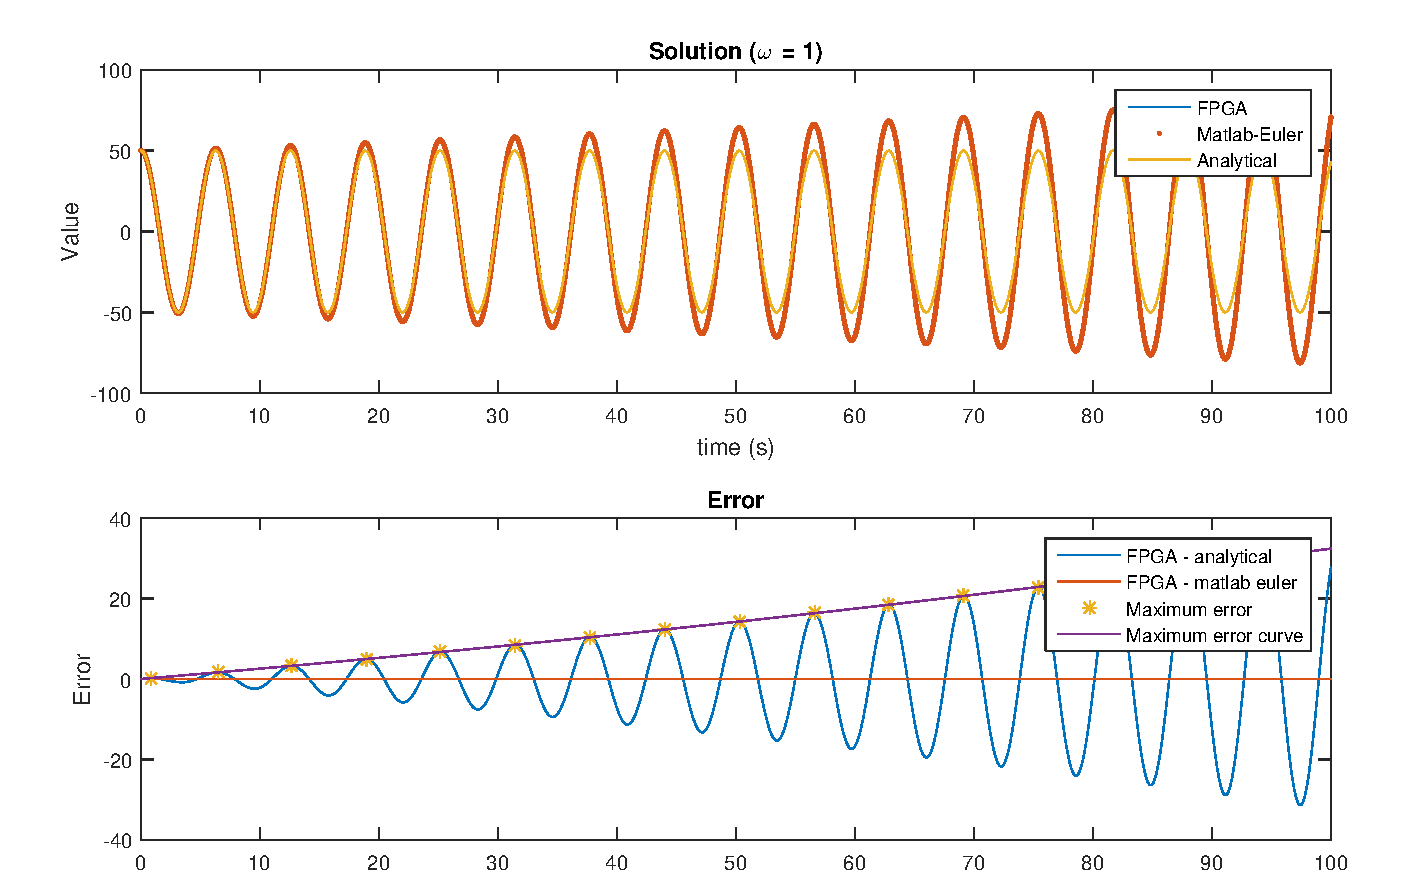
\includegraphics[width=\textwidth]{euler_o1_ts=0,01_os=1}
	\caption{Simple oscillation using Euler's method (h = 0.01)}
	\label{f:euler_o1_ts=0,01_os=1}
\end{figure}

\subsection{First oscillation - initial position}
The plots belonging to the first oscillation (\ref{f:euler_o1_ts=0,01_os=1}) depict three variations on solving the system. Firstly, it contains the solution generated by the FPGA. Secondly, it contains the result of the exact same combination of equation and solver, but implemented in \matlab{}. The only difference between the FPGA and \matlab{} implementation is the number representation. Therefore, if the FPGA solution starts to diverge from the \matlab{} solution the reason has to be the reduced accuracy of the 32-bit fixed point representation used in the FPGA. Internally, \matlab{} uses a (64-bit) double precision floating format \cite{MatlabFloat}, which is guaranteeing a precision of ~15 significant figures for almost all magnitudes supported by the IEEE 754 double precision floating point standard. Lastly, the plot contains the analytical solution of the problem.

The plot shows that the FPGA exhibits the expected behaviour of solving a simple oscillation with Euler's method. Due to the relatively large step size (h = 0.01) the approximation quickly diverges from the analytical solution. The curvature of the solution is always opposite in sign to the solution itself ($x'' = -x$), which results in a self-amplifying effect in the magnitude of the error: an exponential error growth. This was expected, as the exponential dependency was already derived by \cite{DE} in equation \ref{eq:euler_error}. However, this does show that Euler's method is a particularly bad integration scheme for a simple oscillation. It is possible to use \matlab{}s Curve Fitting Tool to fit the equation of the theoretical maximum error of Euler's method to the points of maximum error. After combining some constants, \ref{eq:euler_error} becomes equal to \ref{eq:euler_error_combined}. For $a = 49.75$ and $b = 0.00502$ this equation achieves a fit of $R^{2} = 1$, which is a perfect fit. The error plot and the curve fit of the maximum errors are shown in \ref{f:euler_o1_ts=0,01_os=1}.

\begin{equation}
\label{eq:euler_error_combined}
\text{error}_{\text{euler}}(t) = a (e^{b t} - 1)
\end{equation}

Lastly, the FPGA solution the solution of Euler's method implemented in \matlab{} shows that the error due to the fixed point number representation is clearly insignificant when compared to the intrinsic error in Euler's method: the maximum absolute difference between the two solutions is less than 6\e{-5}.

\subsubsection{Decreasing the time step - improving accuracy?}
The expectation based on \cite{DE} and equation \ref{eq:euler_error} is that the maximum error is indeed proportional to the time step, meaning that a hundred fold decrease of the time step also decreases the error by a factor 100. The maximum error at $t \approx 100$ for $h = 0.01$ was $\approx 30$, whereas the maximum error for $h = 0.0001$ is $\approx 0.2$, which is an improvement of $150 \times$, 50\% more than expected. However, even though the error relative to the analytical solution has decreased, the divergence from the \matlab{} implementation of Euler's algorithm has increased to 8\e{-4}, a factor of 13.

As the time step gets decreased even more, eventually the improvement of having a shorter time step loses out to the reduction the accuracy in the computation. This can be seen very clearly in \ref{f:euler_o1_ts=0,0000001_os=1000}. Featuring a time step of h = 1 \e{-7}, which is approaching the smallest representable value at $2^{-24}$. In this case the \matlab{} implementation is still following the analytical solution with little whereas the solution generated by the FPGA begins to diverge noticeably.

\begin{figure}[h]
	\centering
	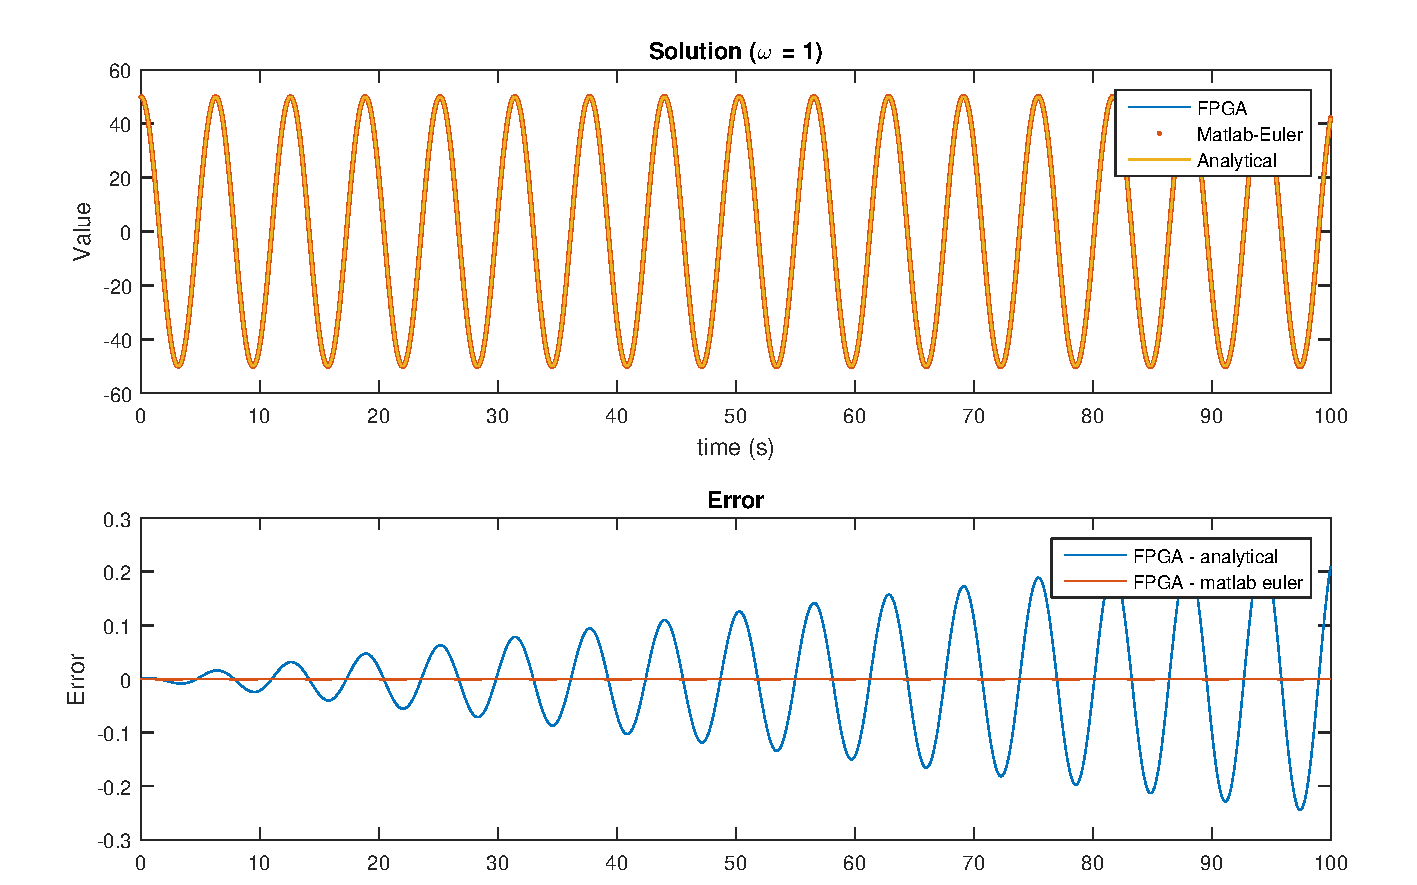
\includegraphics[width=\textwidth]{euler_o1_ts=0,0001_os=100}
	\caption{Simple oscillation using Euler's method with a lower time step (h = 1 \e{-4})}
	\label{f:euler_o1_ts=0,0001_os=100}
\end{figure}

\begin{figure}[h]
	\centering
	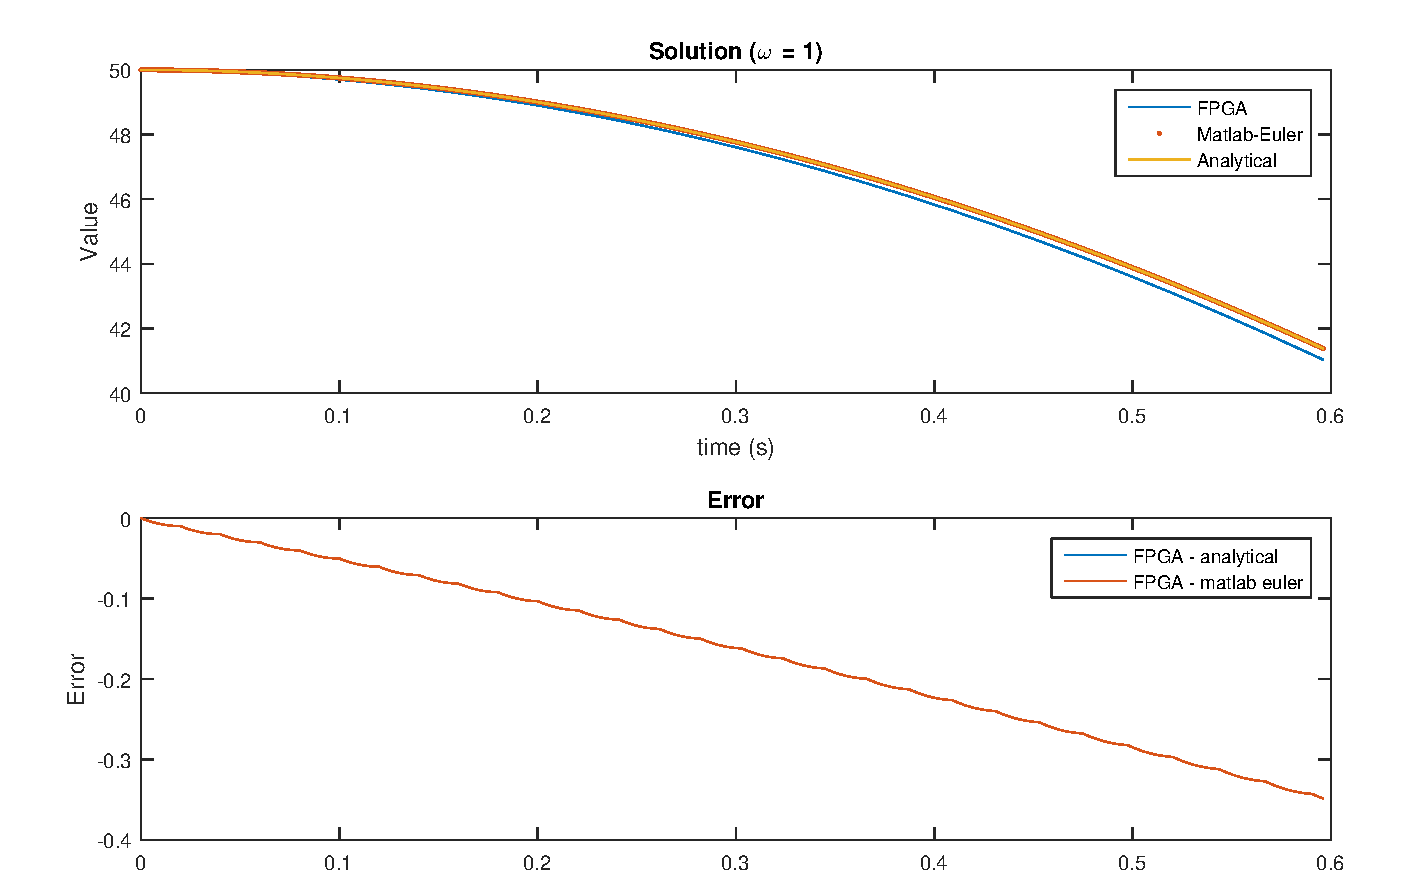
\includegraphics[width=\textwidth]{euler_o1_ts=0,0000001_os=1000}
	\caption{Approaching breakdown due to the fixed point number representation (h = 1 \e{-7})}
	\label{f:euler_o1_ts=0,0000001_os=1000}
\end{figure}

\subsection{Second oscillation - initial velocity}
Similarly to the previous scenario, the error increases exponentially over time and an decrease in time step is approximately proportional to the decrease in error (figure \ref{f:euler_o2_ts=0,001_os=100} and \ref{f:euler_o2_ts=0,00001_os=1000}). However, there is an important difference between the two oscillations: the frequency of oscillation is higher. This has as result that the time step of $h = 0.01$ which worked fine for the oscillation with $\omega = 1$ does not work properly any more: it results in figure \ref{f:euler_o2_ts=0,01_os=1}. This figure shows two interesting phenomena. Firstly, even though \matlab{}s Euler's method does diverge from the analytical solution, it only diverges in magnitude: it stays in phase. However, when looking at the FPGA solution you notice that it diverges from the other two, not only in magnitude but also in phase. The discrepancy in phase between \matlab{} and FPGA indicates that the number representation is the culprit of the shift. 

An attempt to fix this problem was made by changing the relevant part of the matrix from $\left[ \begin{smallmatrix} 0 & 1\\ -4 & 0 \end{smallmatrix} \right]$ to $\left[ \begin{smallmatrix} 0 & 2\\ -2 & 0 \end{smallmatrix} \right]$, which should have the result that the numbers remain smaller internally as the multiplication by 4 is distributed over two multiplications by 2 in separate vector dot products. Even though both matrices result in the same second order equation ($x'' = -4x$) and the eigenvalues are the same, the eigenvalues are different which results in different behaviour for the two matrices.  

\begin{figure}[h]
	\centering
	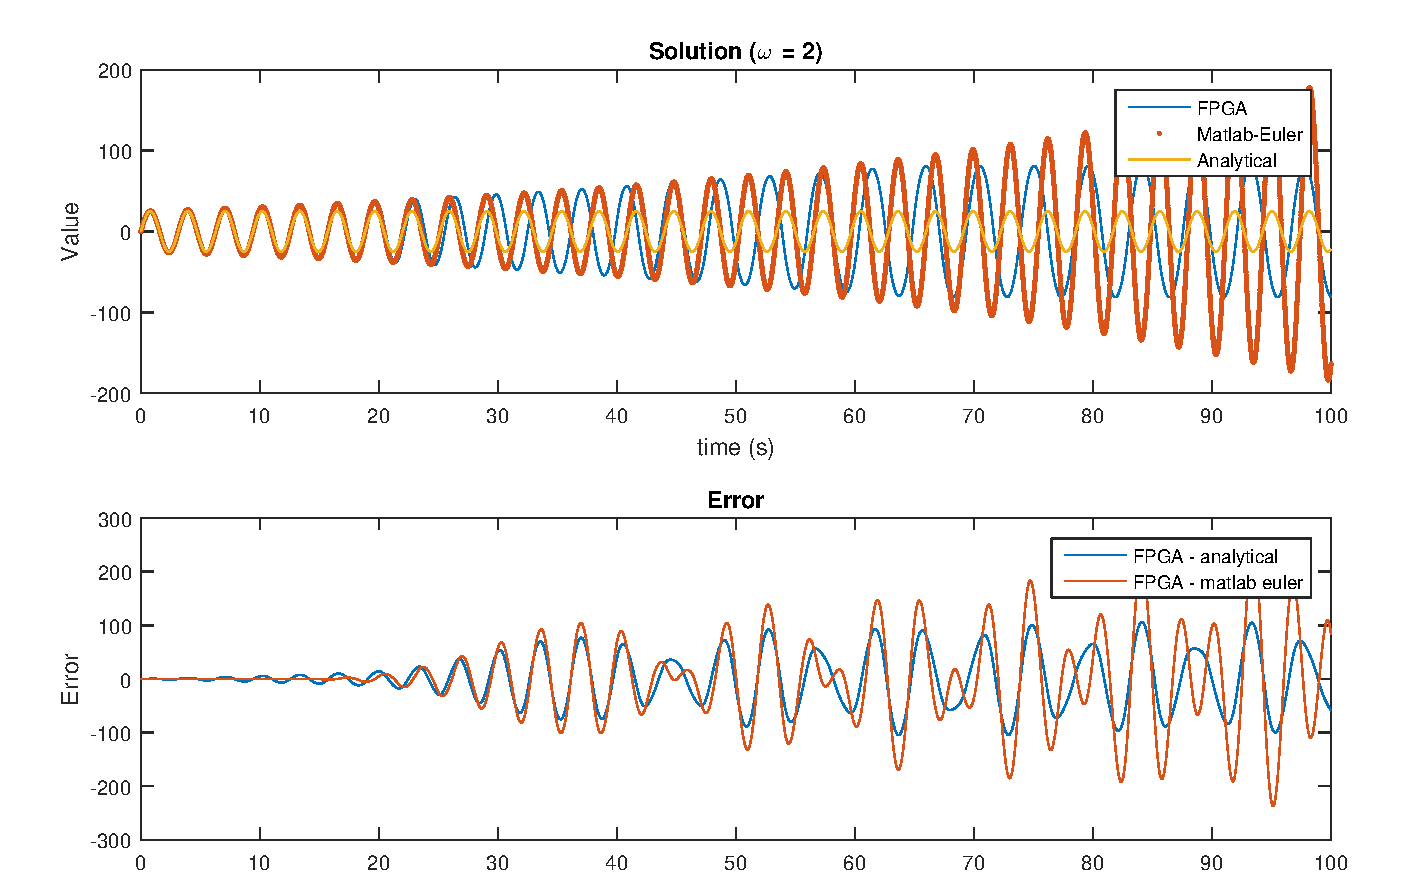
\includegraphics[width=\textwidth]{euler_o2_ts=0,01_os=1}
	\caption{Frequency shifting due to an insufficiently small time step (h = 0.01)}
	\label{f:euler_o2_ts=0,01_os=1}
\end{figure}

\begin{figure}[p]
	\centering
	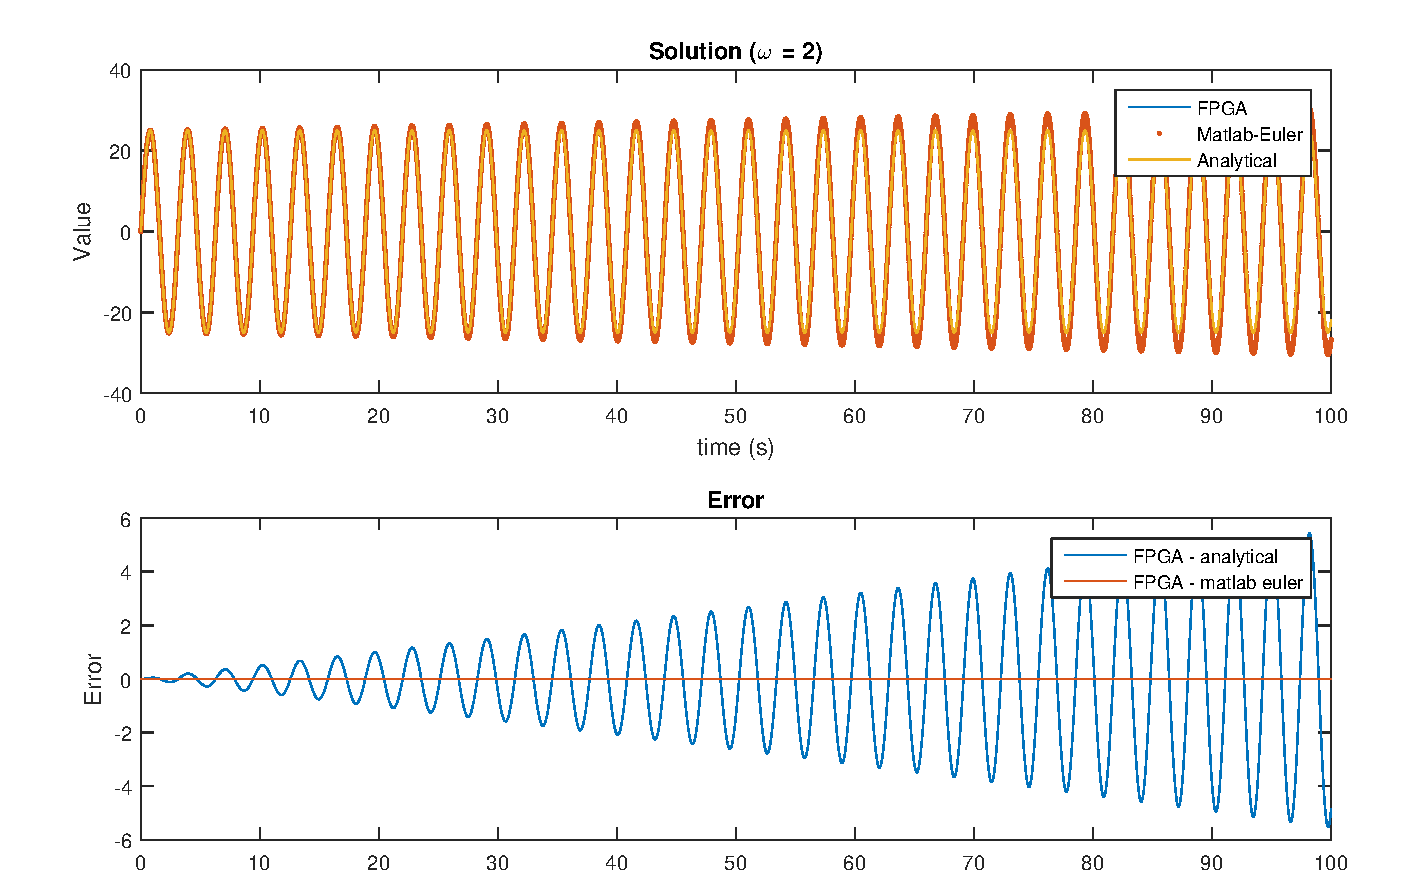
\includegraphics[width=0.95\textwidth]{euler_o2_ts=0,001_os=100}
	\caption{Relatively large time steps result in large errors in the long run (h=0.001)}
	\label{f:euler_o2_ts=0,001_os=100}
\end{figure}

\begin{figure}[p]
	\centering
	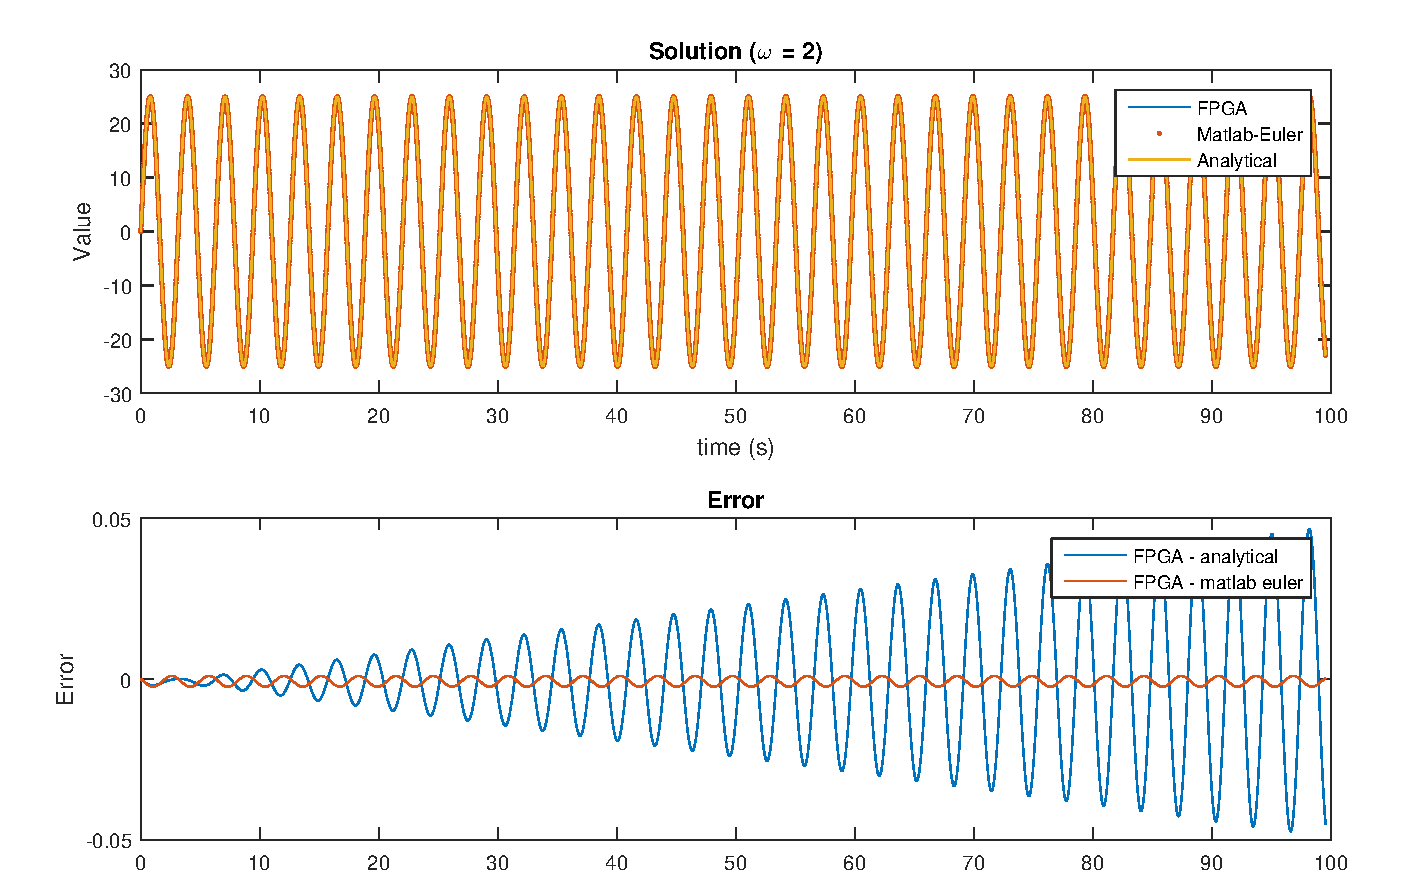
\includegraphics[width=0.95\textwidth]{euler_o2_ts=0,00001_os=1000}
	\caption{But a decrease in time step goes a long way in reducing the error. Note that the error due to the fixed point number representation starts to become significant again, in contrast to figure \ref{f:euler_o2_ts=0,001_os=100} (h = 1 \e{-5})}
	\label{f:euler_o2_ts=0,00001_os=1000}
\end{figure}

\section{Runge-Kutta (second order)}
The testing of the RK2 method uses a different matrix (equation \ref{eq:rk2matrix}) in order to verify the systems capability to correctly solve a system of 4, coupled, first order equations. The matrix has been generated randomly in \matlab{} under the constraint that all eigenvalues are negative. The reason as to why this property is necessary is, again, based on the fixed point number representation. Whenever one of the values (which could even occur internally as part of a vector dot product, invisible to interface) exceeds the allowed range, the result becomes invalid. If all elements in the vector described by the ODE tend towards zero, this problem is less likely to occur (but it might still happen whenever the initial conditions that have been chosen are too large). Furthermore, the added computational steps of RK2 compared to Euler's method have the effect that the time step becomes less important - for the entire range of possible time step values the results and errors are approximately the same (shown in figure \ref{f:rk2_ts=0,01_os=1} and \ref{f:rk2_ts=0,0000005_os=1000}). Lastly, in contrast to the FPGA solution, \matlab{} RK2 and ODE45 do remain close together which, once again, points in the direction of problems stemming from the fixed point numbers.

\begin{equation}
\label{eq:rk2matrix}
\vecb{x}' = \begin{bmatrix} 
2 & 3 & 2 & 0 \\
-5 & -5 & -3 & 1 \\
3 & -1 & -2 & -3 \\
4 & 2 & 2 & -3 \\
\end{bmatrix} \vecb{x} 
\hspace{20pt} \text{with} \hspace{20pt} 
\vecb{x}(t = 0) =\begin{bmatrix} 7 \\ 5 \\ 7 \\ 5 \end{bmatrix} 
\end{equation}

\begin{figure}[p]
	\centering
	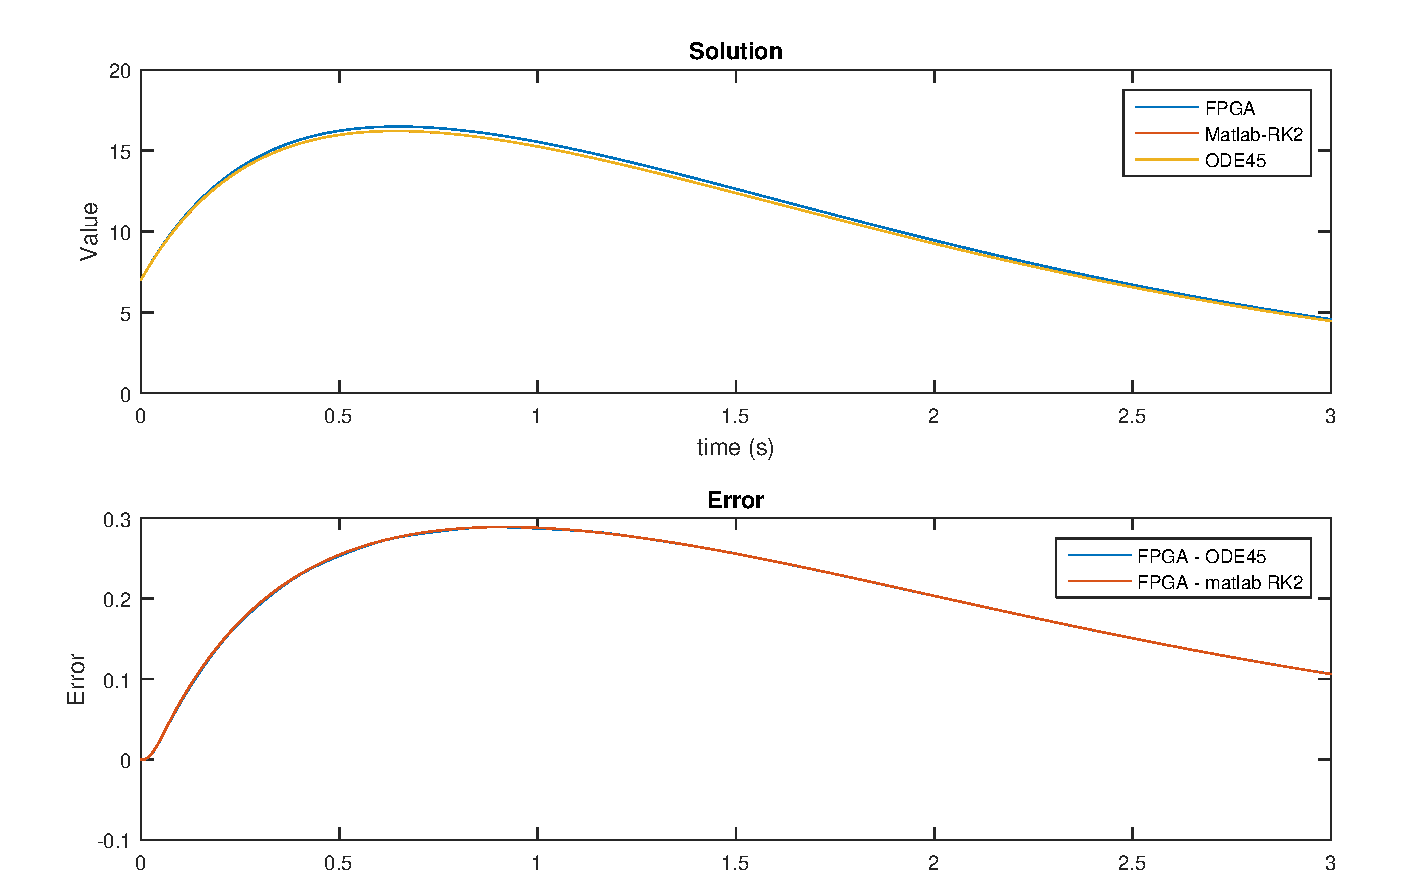
\includegraphics[width=0.95\textwidth]{rk2_ts=0,01_os=1}
	\caption{The largest possible time step has a maximum error of approximately 0.3, for both the comparison with the solution of ODE45 and \matlab{}s RK2 (h=0.01).}
	\label{f:rk2_ts=0,01_os=1}
\end{figure}

\begin{figure}[p]
	\centering
	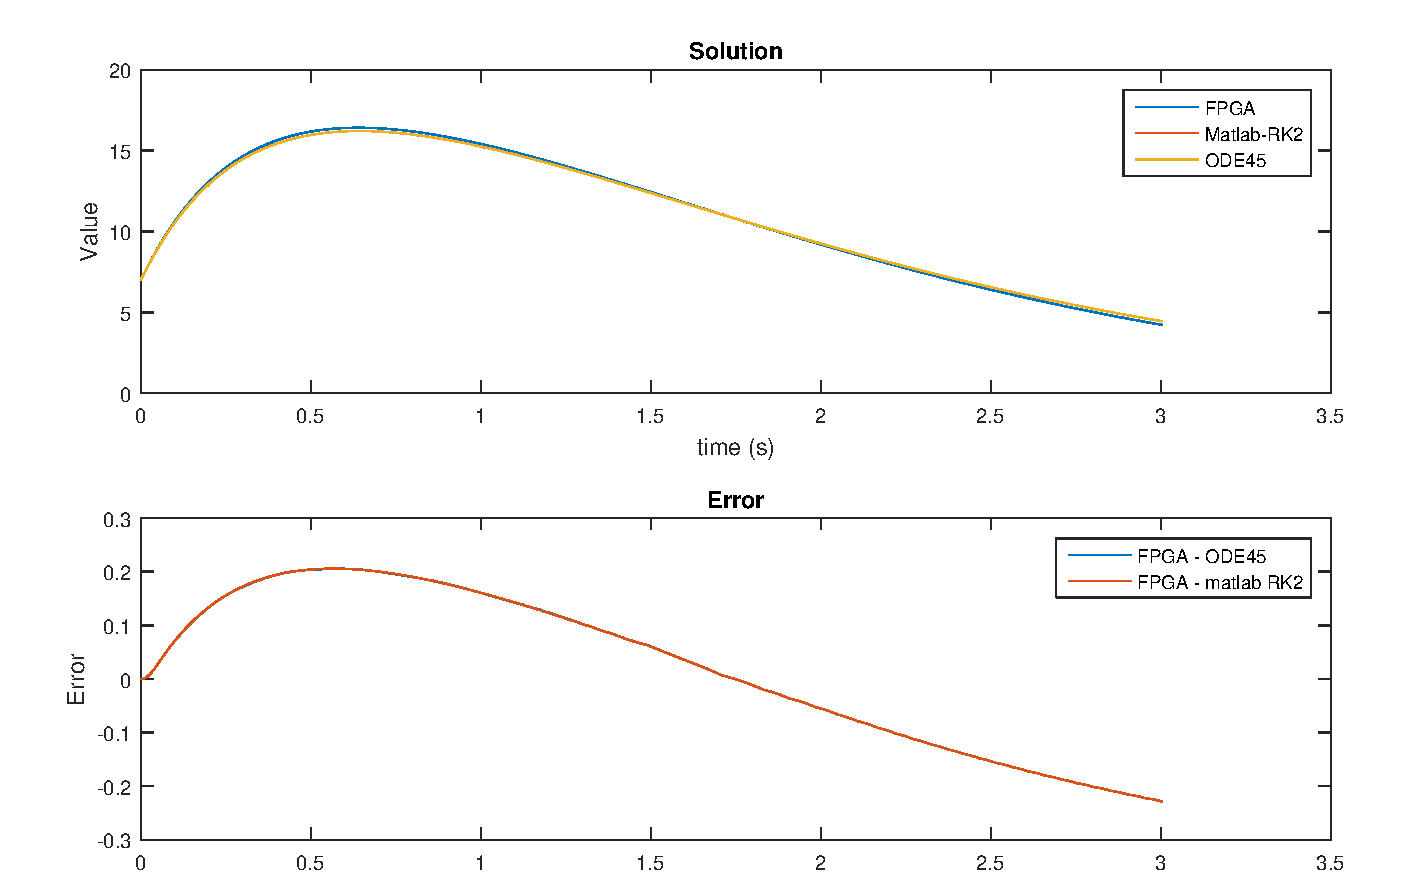
\includegraphics[width=0.95\textwidth]{rk2_ts=0,0000005_os=1000}
	\caption{Considering the other end of the spectrum regarding variety in time steps, the results do not differ significantly enough for the additional amount of work that has to be put in, a factor 20000 (h=5\e{-7}).}
	\label{f:rk2_ts=0,0000005_os=1000}
\end{figure}

\section{Runge-Kutta (fourth order)}
The RK4 integration scheme \footnote{Which took almost 22 hours or 78894 seconds to synthesize.} introduces even more computational steps, which leads to a faster overflow of the internal numbers. This means that at least one of the derivatives overflows almost immediately, which results in plots as shown in figure \ref{f:rk4_ts=0,00001_os=100}.


\begin{figure}[h]
	\centering
	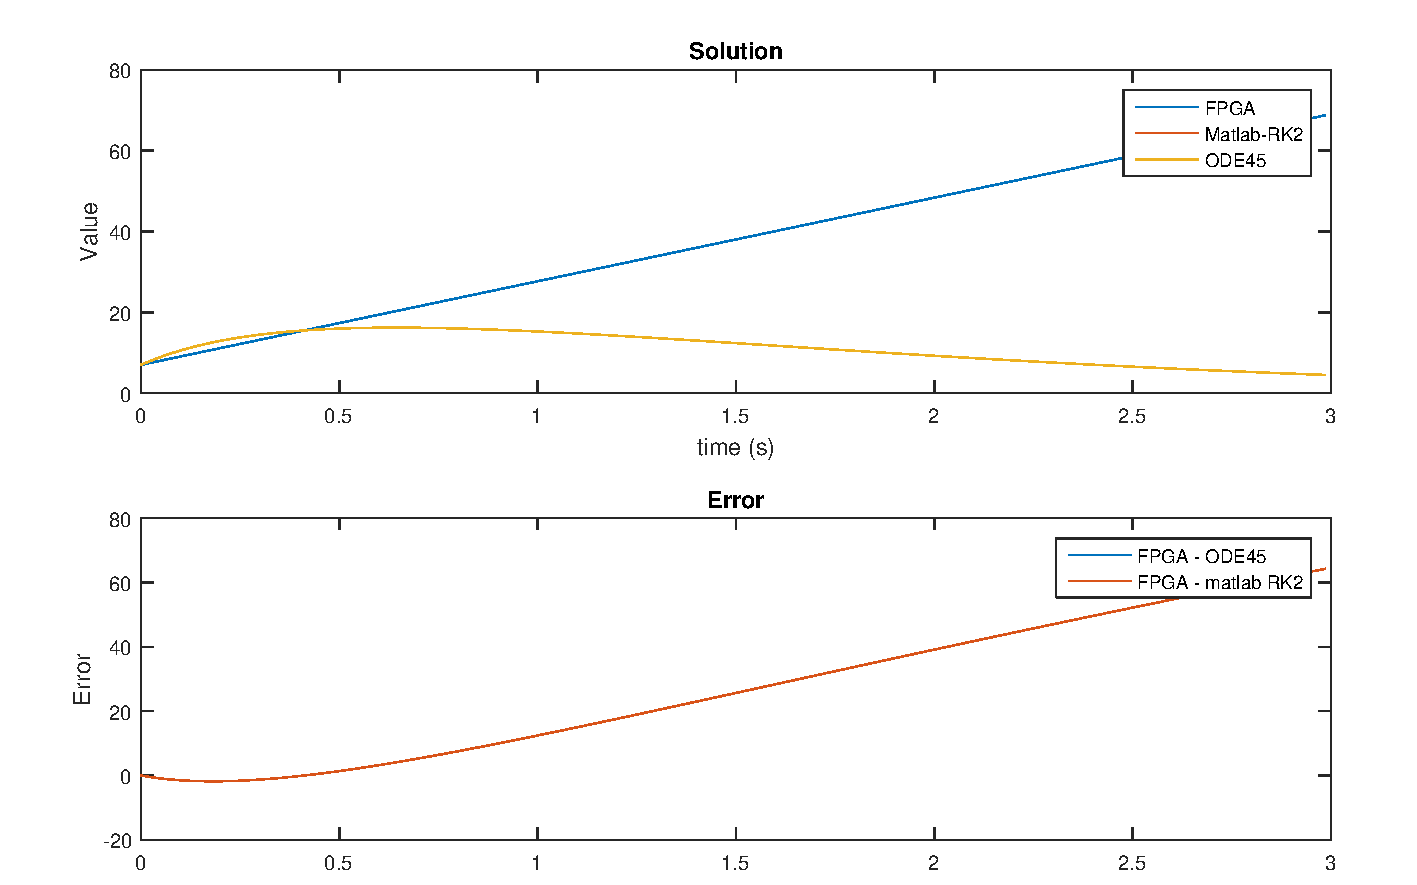
\includegraphics[width=\textwidth]{rk4_ts=0,00001_os=100}
	\caption{For every value of the time step the numbers overflow, causing derivatives to get stuck, resulting in straight lines instead of solutions to ODEs (h=1\e{-5}).}
	\label{f:rk4_ts=0,00001_os=100}
\end{figure}

\section{Euler revisited}
So far it appears that accuracy is inversely proportional to the complexity of the integration scheme, which leads to the question: What accuracy would Euler's method attain for equation \ref{eq:rk2matrix}? Indeed, as shown in figure \ref{f:euler_rv_ts=0,0001_os=10}, Euler's method only reaches maximum errors which are 2 orders of magnitude lower than the best values of the time step for RK2 and of course performs better than RK4 in this scenario. 

\section{Performance - add to conditions to appendix maybe?\textbf{}}
Performance is one of the main reasons why people use FPGAs over implementations in software and therefore one would expect that a properly written FPGA solution outperforms a CPU. The FPGA used for testing in this thesis is a Cyclone V, which, according to \cite{AlteraFPGA}, is meant for "your low-power, cost-sensitive design needs, enabling you to get to market faster". Furthermore, Altera offers two other FPGA families: Stratix and Arria, which both have mentions of delivering high or optimal performance. 

The FPGA runs at a clock speed of 50 MHz and it is capable of executing a single iteration of Euler's method per clock cycle. In theory this would mean that the FPGA is capable of 50\e{6} iterations per second. However, there is still quite some overhead stemming from the system handling the data input and output, which has to wait for the HPS to supply or request the proper information before the FPGA can move on with the computations.

\begin{table}
	\caption{Performance benchmarks: Euler's method}
	\label{t:perfomance}
	\begin{tabular}{l l l l l l}
		Device 	& Iterations& time (s)	& Output every	& Loop bound	& Iterations per second (\e{6}) \\  
		FPGA 	& 1\e{8} 	& 6,53		& 1.000			& 75			& 15,3 	\\
		FPGA 	& 1\e{8} 	& 4,61		& 10.000		& 750			& 21.7 	\\
		FPGA 	& 1\e{8} 	& 4,50		& 100.000		& 7.500			& 22,2 	\\
		FPGA 	& 1\e{8} 	& 4,36		& 100.000.000	& 7.500.000		& 22,9 	\\
		FPGA 	& 1\e{7} 	& 0,77		& 10.000.000	& 750.000		& 13,0 	\\
		FPGA 	& 1\e{6} 	& 0,42		& 1.000.000		& 75.000		& 2,3 	\\
		FPGA 	& 1\e{8} 	& 0,39		& 100.000		& 7.500			& 0,3 	\\
		CPU (i7)& 5\e{7} 	& 20,25		& 50.000.000	& -				& 2,5 	\\
		MATLAB 	& 1\e{7} 	& 303,83	& 10.000.000	& -				& 0,03	\\
	\end{tabular}
\end{table}

\begin{figure}[h!]
	\centering
	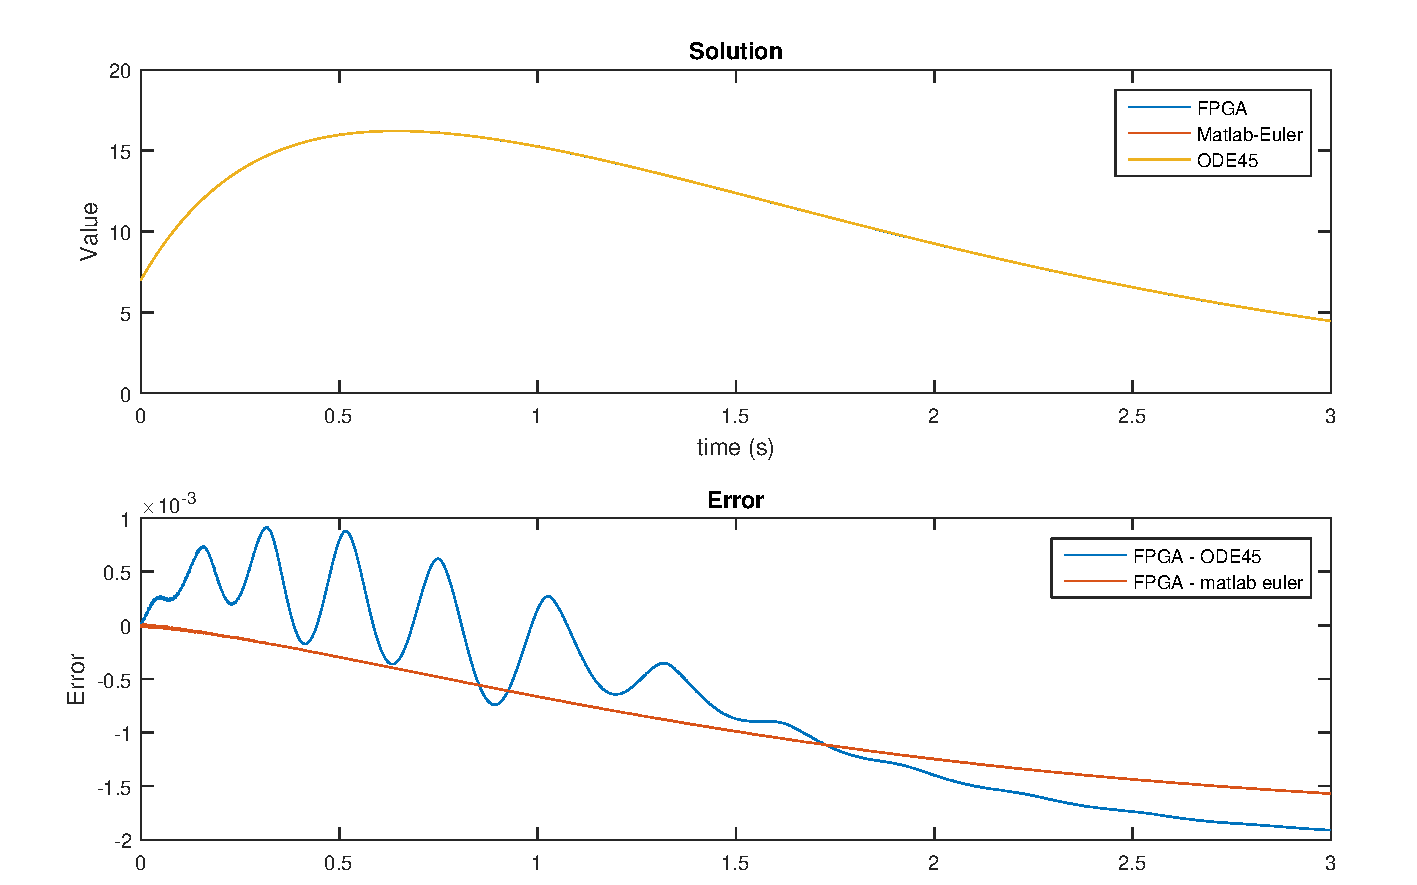
\includegraphics[width=0.9\textwidth]{euler_rv_ts=0,0001_os=10}
	\caption{Simplicity prevails: Euler's method attains better results than RK2 for all different time steps (h=1\e{-4}).}
	\label{f:euler_rv_ts=0,0001_os=10}
\end{figure}





\chapter{Discussion}

\section{sdfassdfsfdf}
\chapter{Conclusion}

\section{Keep in mind the number representation !! AVOID OVERFLOW}

% ********************************** Back Matter *******************************
% Backmatter should be commented out, if you are using appendices after References
%\backmatter

% ********************************** Bibliography ******************************
\begin{spacing}{0.9}

% To use the conventional natbib style referencing
% Bibliography style previews: http://nodonn.tipido.net/bibstyle.php
% Reference styles: http://sites.stat.psu.edu/~surajit/present/bib.htm

\bibliographystyle{plainnat} % use this to have URLs listed in References
%\clearpage
\bibliography{References/references} % Path to your References.bib file


% If you would like to use BibLaTeX for your references, pass `custombib' as
% an option in the document class. The location of 'reference.bib' should be
% specified in the preamble.tex file in the custombib section.
% Comment out the lines related to natbib above and uncomment the following line.

%\printbibliography[heading=bibintoc, title={References}]


\end{spacing}

% ********************************** Appendices ********************************

\begin{appendices} % Using appendices environment for more functunality

\chapter{Haskell source code for numerical solutions of ODEs} 
\label{app:haskellsolver}
\lstset{style=haskellStyle}

\lstinputlisting[caption=Solver.hs]{../haskell/Solver.hs}
\lstinputlisting[caption=SolverTypes.hs]{../haskell/SolverTypes.hs}
\lstinputlisting[caption=SolverEquations.hs]{../haskell/SolverEquations.hs}

\lstinputlisting[caption=SolverPresets.hs]{../haskell/SolverPresets.hs}
\lstinputlisting[caption=SolverHelper.hs]{../haskell/SolverHelper.hs}
\lstinputlisting[caption=SolverPlotter.hs]{../haskell/SolverPlotter.hs}
\chapter{Project structure}
\label{app:project_structure}
The entire project is hosted on GitHub - \url{https://github.com/Gladdy/numerical-fpga-thesis}

\dirtree{%
	.1 .
	.2 benchmark \DTcomment{Performance comparisons to C++ and Haskell}.
	.3 c++.
	.3 haskell.
	.2 clash.
	.3 vhdl.
	.4 Solver \DTcomment{The \clash{}-generated VHDL}.
	.2 control \DTcomment{C++ for controlling the FPGA from the HPS}.
	.2 haskell.
	.2 images \DTcomment{Ready-made numerical solver images for the Cyclone V FPGA}.
	.2 kernel \DTcomment{Bootloader and scripts for linux kernel generation}.
	.2 literature.
	.2 minified \DTcomment{Sample project for easy modifictation}.
	.3 clash.
	.3 control.
	.3 sockit.
	.3 minified.zip.
	.2 sockit \DTcomment{Full quartus project}.
	.2 thesis.
	.2 verification \DTcomment{\matlab{} result verification scripts}.
}
\chapter{Handling data IO}
\label{app:data_io}
Due to the library code written, the process of controlling the FPGA could not be more simple. Listing \ref{lst:control_main} shows the user-side interface, in which the comments have made any further explanation obsolete. The background library written handles all low-level processes, for instance writing directly to a memory location and converting the doubles to fixed-point numbers. Comments have been added to explain the code in the important sections. The code is very object-oriented, improving clarity and comprehensibility. The sources can be found in the GitHub repository at \url{https://github.com/Gladdy/numerical-fpga-thesis}  

\lstinputlisting[language=C++, caption=Controlling the FPGA,label=lst:control_main]{../control/main.cpp}


\chapter{Toolchain integration}
\label{app:toolchain_integration}

A single script has integrated the entire toolchain, from the process of generating HDL in \clash{} to deploying and running the program on the FPGA. This script has several dependencies, so make sure that all these commands are available in your \code{\$PATH}.

\begin{itemizens}
\item \emph{GnuWin32} - The script is written for the \code{bash} shell and has been tested using the GNUWin32 implementation. It also depends on \code{sed}, \code{ssh}, \code{scp}, \code{rm} and \code{cp}, \code{mv}, which are not available by default on Windows.
\item \emph{Quartus} - For compiling the VHDL into a \code{.sof} (SDRAM Object File) and converting this into a \code{.rbf} (Raw Binary File), used to flash the FPGA.
\item \emph{A linux installation running on the SoC} Make sure that the hostname and the port for SSH access are specified properly and the board is running a correct version of Linux. The scripts which automate the set-up of a proper Linux image are also located in the repository, in the folder \code{./kernel}.
\end{itemizens}

\lstinputlisting[language=bash, caption=Full integration of the toolchain]{../run.sh}
\chapter{Performance benchmark}
\label{app:performance_benchmark}


\end{appendices}

% *************************************** Index ********************************
\printthesisindex % If index is present

\end{document}
